%%================================================
%% Filename: chap04.tex
%% Encoding: UTF-8
%% Author: Yuan Xiaoshuai - yxshuai@gmail.com
%% Created: 2012-04-28 00:15
%% Last modified: 2019-11-06 17:39
%%================================================
\chapter{基于特征融合的增量学习异常流量检测模型}
% \chapter{基于多模态特征融合的增量学习方案}
\label{cha:ResNet-BiGRU}

由于传统的网络攻击检测方法不能综合分析网络流量数据中的空间特征与时序特征,网络攻击检测的准确性仍有很大的提升空间。
因此,本文设计并提出了一个基于残差网络与双向门控循环单元的多模态特征融合模型(ResNet-BiGRU based Multimodal Fusio,RB-MF),旨在充分挖掘流量数据时空特征的同时,对其综合分析,进一步提高模型准确率。
此外,针对传统攻击检测技术在应对新型攻击时表现出的检测能力不足、难以适应攻击模式不断变化的问题,本文在所提模型RB-MF的基础上进一步设计并实现了一个增量学习方案——基于特征融合模型的增量学习方案。
本方案在保留模型原有知识的基础上,使其具备持续适应和学习新攻击模式的能力,进而逐步适应日新月异的攻击环境,确保安全防护的时效性和准确性。
图~\ref{fig:attack_detecion_model}~描述了本文方案的工作原理和流程。
\begin{figure}[h]
	\centering
	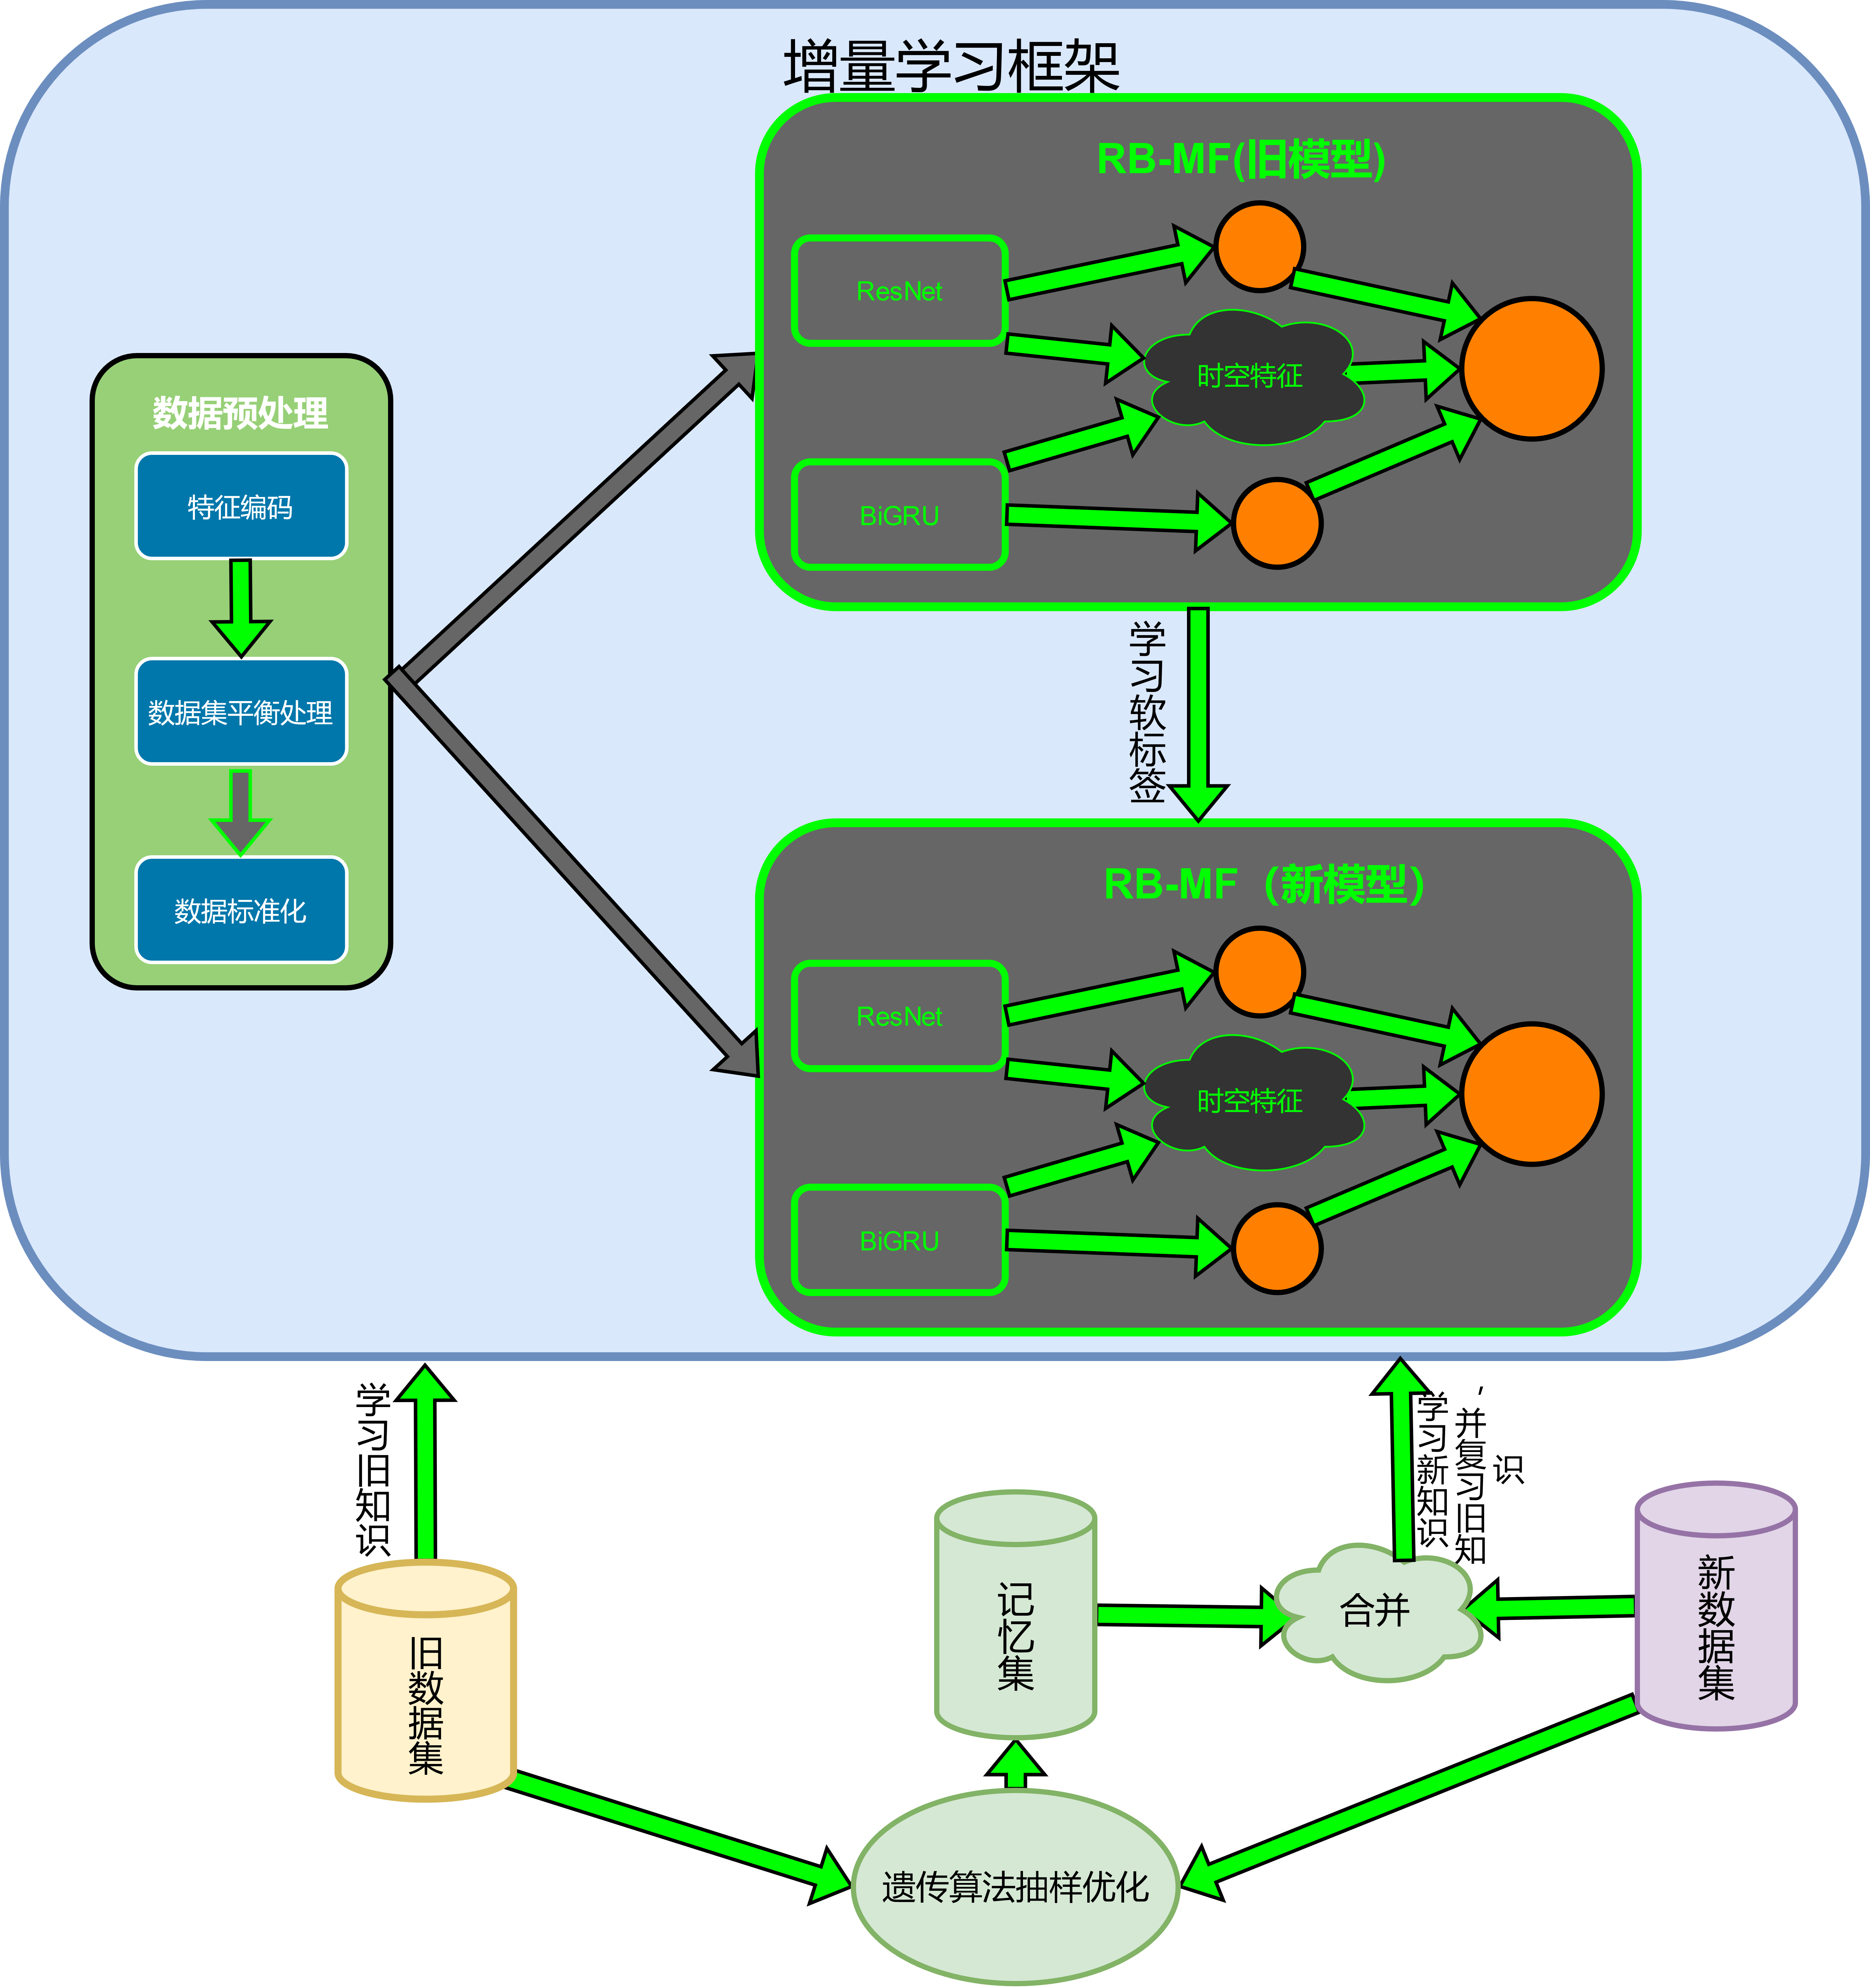
\includegraphics[width = 0.74\textwidth]{chapter_4.drawio.png}
	\caption{基于多模态特征融合的增量学习方案原理及流程}
	\label{fig:attack_detecion_model}
\end{figure}

基于多模态特征融合模型的增量学习方案由以下四个关键部分构成:首先是RB-MF模型的结构设计,其次是数据集的预处理流程,再次是RB-MF模型的增量学习策略,最后是记忆集的抽样优化方法。
首先,第一部分是本文接下来将要提出的RB-MF模型的设计与实现,该模型能够综合分析流量数据集的时空特征,在攻击检测准确率方面具有很好的表现。
第二部分对数据集进行预处理,确保RB-MF模型能够顺利地进行训练和测试。
第三部分在RB-MF模型完成旧任务数据的训练后,结合iCaRL\cite{rebuffi2017icarl}策略使RB-MF模型具备持续学习和适应新环境的能力。
最后一部分则利用遗传算法实现iCaRL策略中记忆集的分层抽样优化,使得RB-MF模型在固定大小的记忆集上最大化记忆能力。

\section{基于特征融合的异常流量检测模型}
% 网络通信涉及复杂的交互模式,包括客户端与服务器之间的请求响应、数据传输过程中的拥塞控制等。
% 这些交互在空间上体现为数据包的具体内容,如源IP地址、目标IP地址、端口号、协议类型等,这些信息在数据包的特定位置以特定格式存在,形成了数据的“空间”结构。
% 在时间上则表现为交互的顺序和持续时间。\par
该模型的原理是通过多模态特征融合技术将ResNet以及BiGRU进行融合,从而综合分析网络流量数据中的时空特性,提升决策性能。
其具体流程为,首先,ResNet提取网络流量数据中的深层次空间特征,BiGRU则捕捉流量数据时序特征的前后依赖关系。
接着,结合这两个特征形成混合的“时空特征”。
最后,综合ResNet和BiGRU的决策输出以及“时空特征”,结合三者,产生最终的决策输出。
\subsection{多模态特征融合设计}
多模态特征融合是一种将来自不同来源或类型(模态)的数据集成在一起的过程,目的是改善决策过程提高预测准确性。
这些不同模态的数据可能包括文本、图像、视频、音频和传感器数据等。
在机器学习和深度学习领域,多模态特征融合已成为一个重要的研究领域,尤其是在那些需要综合处理不同类型数据的应用中,如自然语言处理、计算机视觉、语音识别和人机交互等。
融合策略通常可以分为早期融合、晚期融合、混合融合三种类型\cite{hejunandzhangcaiqing}。\par

早期融合(如图~\ref{fig:MultimodalFusio} (a)~所示),也被称为特征级融合,其核心思想是在模型的某个中间层将不同模态的特征进行集成。
这种策略充分利用了深度学习模型在捕捉和利用模态间交互作用方面的能力。\par

晚期融合(如图~\ref{fig:MultimodalFusio} (b)~所示)则采取了另一种思路。
在这种策略中,每个模态都单独处理并产生决策,而最终的融合则发生在决策层面,通常通过投票机制、平均值计算或是基于学习的加权组合等方式来实现。
晚期融合的优点在于能够保持模态间的独立性,适用于模态间关联较弱的情况。\par

混合融合(如图~\ref{fig:MultimodalFusio} (c)~所示)策略则更为灵活,它结合了早期融合和晚期融合的优点,旨在在特征提取和决策过程中充分利用各种融合方法的优势。
例如,一个混合融合框架可能同时利用早期融合来捕捉模态间的直接联系,同时借助晚期融合来维持某些模态的独立性,从而确保信息处理的全面性和准确性。
这种策略不仅提升了融合效果,也增强了模型的鲁棒性和泛化能力。\par

\begin{figure}[h]
	\centering
	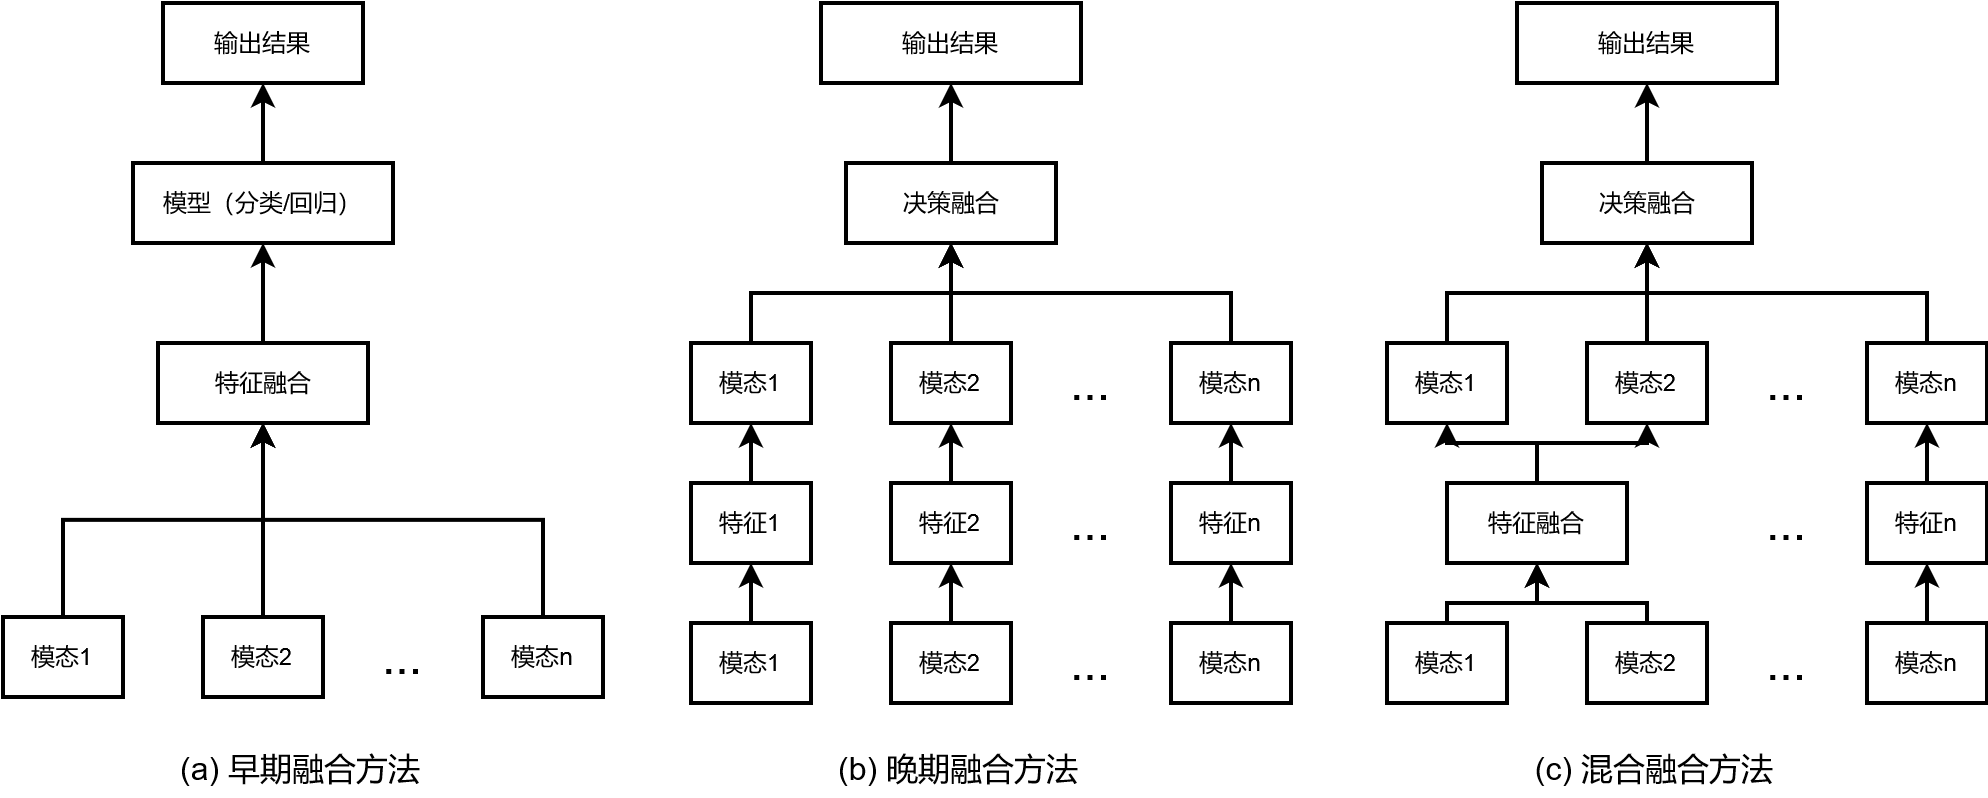
\includegraphics[width = \textwidth]{MultimodalFusion.drawio.png}
	\caption{3种多模态特征融合方法}
	\label{fig:MultimodalFusio}
\end{figure}


早期融合的效果在很大程度上取决于对模态特性的理解和模型结构设计。
然而,由于不同模态数据的多样性和复杂性,早期融合可能并不总是适用于所有类型的多模态数据。
在某些情况下,不恰当的融合方式可能会导致信息丢失或模型性能下降。
晚期融合虽然能够保持模态之间的独立性,但由于每个模态是独立处理的,它可能无法充分捕获模态之间的深层次相互作用。
此外,晚期融合通常在决策层面进行,这在一定程度上限制了对不同模态特征之间更细粒度关系的探索和利用。
相比之下,混合融合策略通过结合早期融合和晚期融合的优点,为模型设计提供了更大的灵活性和适应性。
它能够在不同的层级和阶段整合不同模态的信息,从而最大化地利用不同模态之间的互补性和关联性。这种策略不仅能够捕获模态之间的直接特征信息,还能够挖掘深层次的相互作用信息,进一步提升模型的性能。\par



因此,本文将会利用混合融合策略来整合ResNet和BiGRU模型的优势。
首先,本文将分别利用ResNet和BiGRU来从网络流量数据集中提取空间特征和时序特征。
ResNet的强大之处在于其深度结构和残差连接,使其能够捕捉到网络流量数据中的复杂空间模式;而BiGRU则通过其双向结构,有效地捕获了时序数据中的长期依赖关系。
接着,为了高效且有效地融合这两种特征,本文采用联合架构。
联合架构有两种融合方法,即“加”联合方法和“乘”联合方法。
“加”联合方法,也称为加法融合,是一种直观且计算效率高的方式。它通过对不同模态的特征向量进行加权和或简单的相加操作来融合特征。
这种方法基于一个假设,即不同模态的特征贡献可以直接相加,从而形成一个综合的特征表示。
加法融合不仅易于实现,而且能够保留原始特征中的大部分信息,同时减少了计算复杂度。
加法融合可以表示为:
\begin{equation}
	z = f(w_1^Tv_1 + w_2^Tv_2+ \dots + w_n^Tv_n)
\end{equation}
\begin{flushleft}
	\renewcommand\arraystretch{1.25}
	\begin{tabularx}{\textwidth}{@{}>{\normalsize\rm}l@{\quad}>{\normalsize\rm}l@{——}>{\normalsize\rm}X@{}}
		式中 & $z$ & 共享语义子空间的输出结果;                                              \\
		     & $N$ & 类别总数;                                                              \\
		     & $v$ & 各模态的输入;                                                          \\
		     & $w$ & 权重,下标表示不同的模态,通过映射$f$将所有子模态语义转换到共享子空间。 \\
	\end{tabularx}\vspace{.5ex}
\end{flushleft}


“乘”联合方法,或乘法融合,涉及到对不同模态的特征进行乘积操作。
这种方法基于这样的假设:一个模态的特征可以通过与另一模态的特征进行乘积来增强或抑制重要的信号。
乘法联合可以用以下公式表示:
\begin{equation}
	z = \begin{bmatrix}v^1 \\1\\\end{bmatrix} \otimes \begin{bmatrix}v^2 \\1\\\end{bmatrix} \otimes \dots \otimes \begin{bmatrix}v^n \\1\\\end{bmatrix}
\end{equation}
\begin{flushleft}
	\renewcommand\arraystretch{1.25}
	\begin{tabularx}{\textwidth}{@{}>{\normalsize\rm}l@{\quad}>{\normalsize\rm}l@{——}>{\normalsize\rm}X@{}}
		式中 & $z$       & 融合张量后的结果输出; \\
		     & $v$       & 不同的模态;           \\
		     & $\otimes$ & 外积算子。             \\
	\end{tabularx}\vspace{.5ex}
\end{flushleft}



尽管“加”联合方法具有简单性和易实现性的优势,但它可能因特征向量语义组合的局限性而导致后期语义信息的丢失,进而影响模型性能。
相对而言,“乘”联合方法通过张量计算的方式,能够更加深入地融合特征语义,弥补“加”联合方法的不足\cite{hejunandzhangcaiqing}。
因此,为了更全面地融合ResNet和BiGRU提取的空间与时序特征,本文将采用“乘”联合方法来进行特征融合。
这种方法能够确保特征语义在融合过程中得到充分保留和增强,从而有望提高模型的准确性和鲁棒性。\par

最终,本文所构建的融合架构如图~\ref{fig:ResNet-BiGRU-Fusion}~所示。
\begin{figure}[htbp]
	\centering
	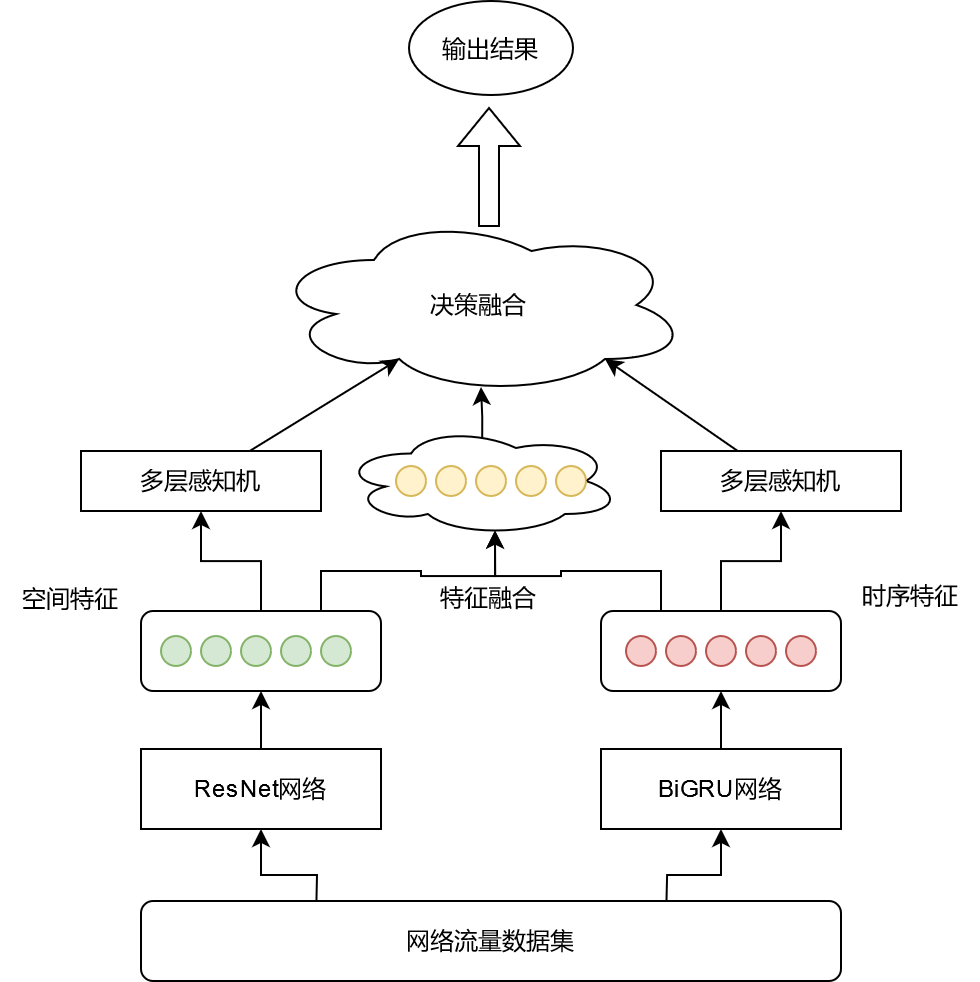
\includegraphics[width = 0.7\textwidth]{ResNet-BiGRU-Fusion.drawio.png}
	\caption{ResNet-BiGRU特征融合设计}
	\label{fig:ResNet-BiGRU-Fusion}
\end{figure}
该架构充分利用了混合融合策略的优势,通过结合ResNet和BiGRU的特征提取能力,并采用“乘”联合方法进行特征融合,为网络流量分析等相关任务提供了强大的支持。

\subsection{模型网络结构设计}
本文的融合模型核心在于残差网络与双向门控循环单元网络的结合,并通过独特的多模态特征融合策略实现两者间的有效协同。
% 本文的融合模型主要由一个残差网络以及一个双向门控循环单元网络以及它们之间的多模态特征融合方式构成。
其中,残差模型主要包括两种类型的残差块:conv\_block(卷积残差块)和identity\_block(恒等残差块)。
这两种块的设计旨在解决深度神经网络训练中常见的梯度消失问题,从而使网络能够在增加深度的同时保持训练的有效性和稳定性。
conv\_block负责调整输入特征图的维度,以匹配块输出时的维度变化。
它通过在残差路径中引入具有步长的卷积操作来实现降维,并通过额外的卷积层来调整通道数,从而使得主路径上的特征图尺寸与残差路径上的输出能够相匹配。
这种设计使得网络能够在增加深度的同时,适应更高层的特征表示。
identity\_block则在不需要改变输入特征图维度时使用,主要用于网络的深层部分,用以加深网络深度提高模型的性能。\par

残差模型以15x15\footnote{特征编码后,数据维度变为(214,1)。为进行2D卷积,本文将其调整为(15,15,1)并进行了零填充。}的二维输入数据开始,紧接着是一个初始卷积层,该层使用64个3x3大小的滤波器,并应用“same”填充,以保持输出特征图的尺寸。
此外,这一层使用L2正则化以防止过拟合,并通过批归一化(BatchNormalization)和ReLU激活函数对特征进行标准化和非线性化处理。

接下来,模型通过两个阶段的残差块处理特征:

\begin{enumerate}[label=\arabic*)]
	\item 第一阶段包含一个conv\_block和一个identity\_block,分别用于特征图的尺寸和深度调整以及模型深度的增加。
	\item 第二阶段则起始于另一个conv\_block,随后是两个identity\_block,以进一步增强模型的特征提取能力。
\end{enumerate}
每个卷积层都配备了L2正则化,且所有残差块后都跟随批归一化和ReLU激活函数,以促进有效训练并避免梯度问题。

在经过残差块序列处理后,模型使用平均池化层(AveragePooling2D)来减小特征图的尺寸,随后是一个Dropout层,以0.5的比率随机断开输入单元,降低过拟合的风险。
最后,模型将处理后的特征展平,为与BiGRU的时序特征融合做准备。表~\ref{tab:resnet_description}~是该残差网络的具体结构。


\begin{table}[h]
	\caption{残差网络模型结构}
	\label{tab:resnet_description}
	\centering
	\begin{tabular}{c|c|c}
		\hline
		Layer name                & Output size                              & ResNetPart             \\
		\hline
		conv1                     & $15 \times 15$                           & $3\times3$, 64, stride 1 \\
		\hline
		% 使用multirow和mbox命令来确保矩阵居中
		\multirow{4}{*}{conv2\_x} & \multirow{4}{*}{\centering $8 \times 8$} &
		\multirow{4}{*}{$\left[\begin{array}{c}
						1 \times 1, 64 \\
						3 \times 3, 64 \\
						1 \times 1, 256
					\end{array}\right] \times 2$ , stride 2}                  \\
		                          &                                          &                          \\
		                          &                                          &                          \\
		                          &                                          &                          \\
		\hline
		\multirow{4}{*}{conv3\_x} & \multirow{4}{*}{\centering $8 \times 8$} &
		\multirow{4}{*}{$\left[\begin{array}{c}
						1 \times 1, 64 \\
						3 \times 3, 64 \\
						1 \times 1, 256
					\end{array}\right] \times 2$, stride 1}                   \\
		                          &                                          &                          \\
		                          &                                          &                          \\
		                          &                                          &                          \\
		\hline
		avg\_pool                 & $1 \times 1$                             & AvgPool $2 \times 2$     \\
		\hline
		flatten                   & 1,1264                                   &                          \\
		\hline
		dropout                   &                                          & Dropout(0.5)             \\
		\hline
	\end{tabular}
\end{table}


对于BiGRU模型,第一层包含64个单元,用于捕捉序列数据的时序依赖关系,并保留每个时间步的输出。这一设计旨在充分提取序列中的动态特征。
为了降低模型过拟合的风险,模型在第一层BiGRU后引入了一个10\%的dropout层,通过随机丢弃部分特征连接来增强模型的泛化能力。
随后,数据进入第二个BiGRU层,该层拥有32个单元,专注于捕捉更深层次的时序信息。与第一层不同,这一层仅输出最后一个时间步的结果,以捕捉序列的整体趋势。
随后是另一个10\%的dropout层,以进一步减少过拟合。
值得注意的是,为了将BiGRU层的特征输出与ResNet模型的特征进行合并,在这个结构中也同样并没有加入全连接层(Dense layer)作为输出。\par


最终,RB-MF将从ResNet模型和BiGRU模型中分别提取特征,并通过特定的融合策略进行合并。
此外,为了与BiGRU的输出维度相匹配,RB-MF将ResNet的输出从11264维通过适当的映射降维至64维。
随后,采用元素乘法操作将两种模型的特征进行融合,确保不同模态的信息能够相互补充。
在特征融合后,RB-MF将ResNet和BiGRU的决策输出与融合特征合并成一个统一的张量。这一张量随后通过一个额外的Dense层进行进一步处理,最终输出分类决策。
通过这一设计,RB-MF能够充分利用ResNet和BiGRU各自的优势,并通过混合融合策略实现多模态特征的有效整合。

图~\ref{fig:hyber_model_struct}~是这个混合模型的整体架构,表~\ref{tab:model_params}~是混合模型的参数数量。
\begin{figure}[h]
	\centering
	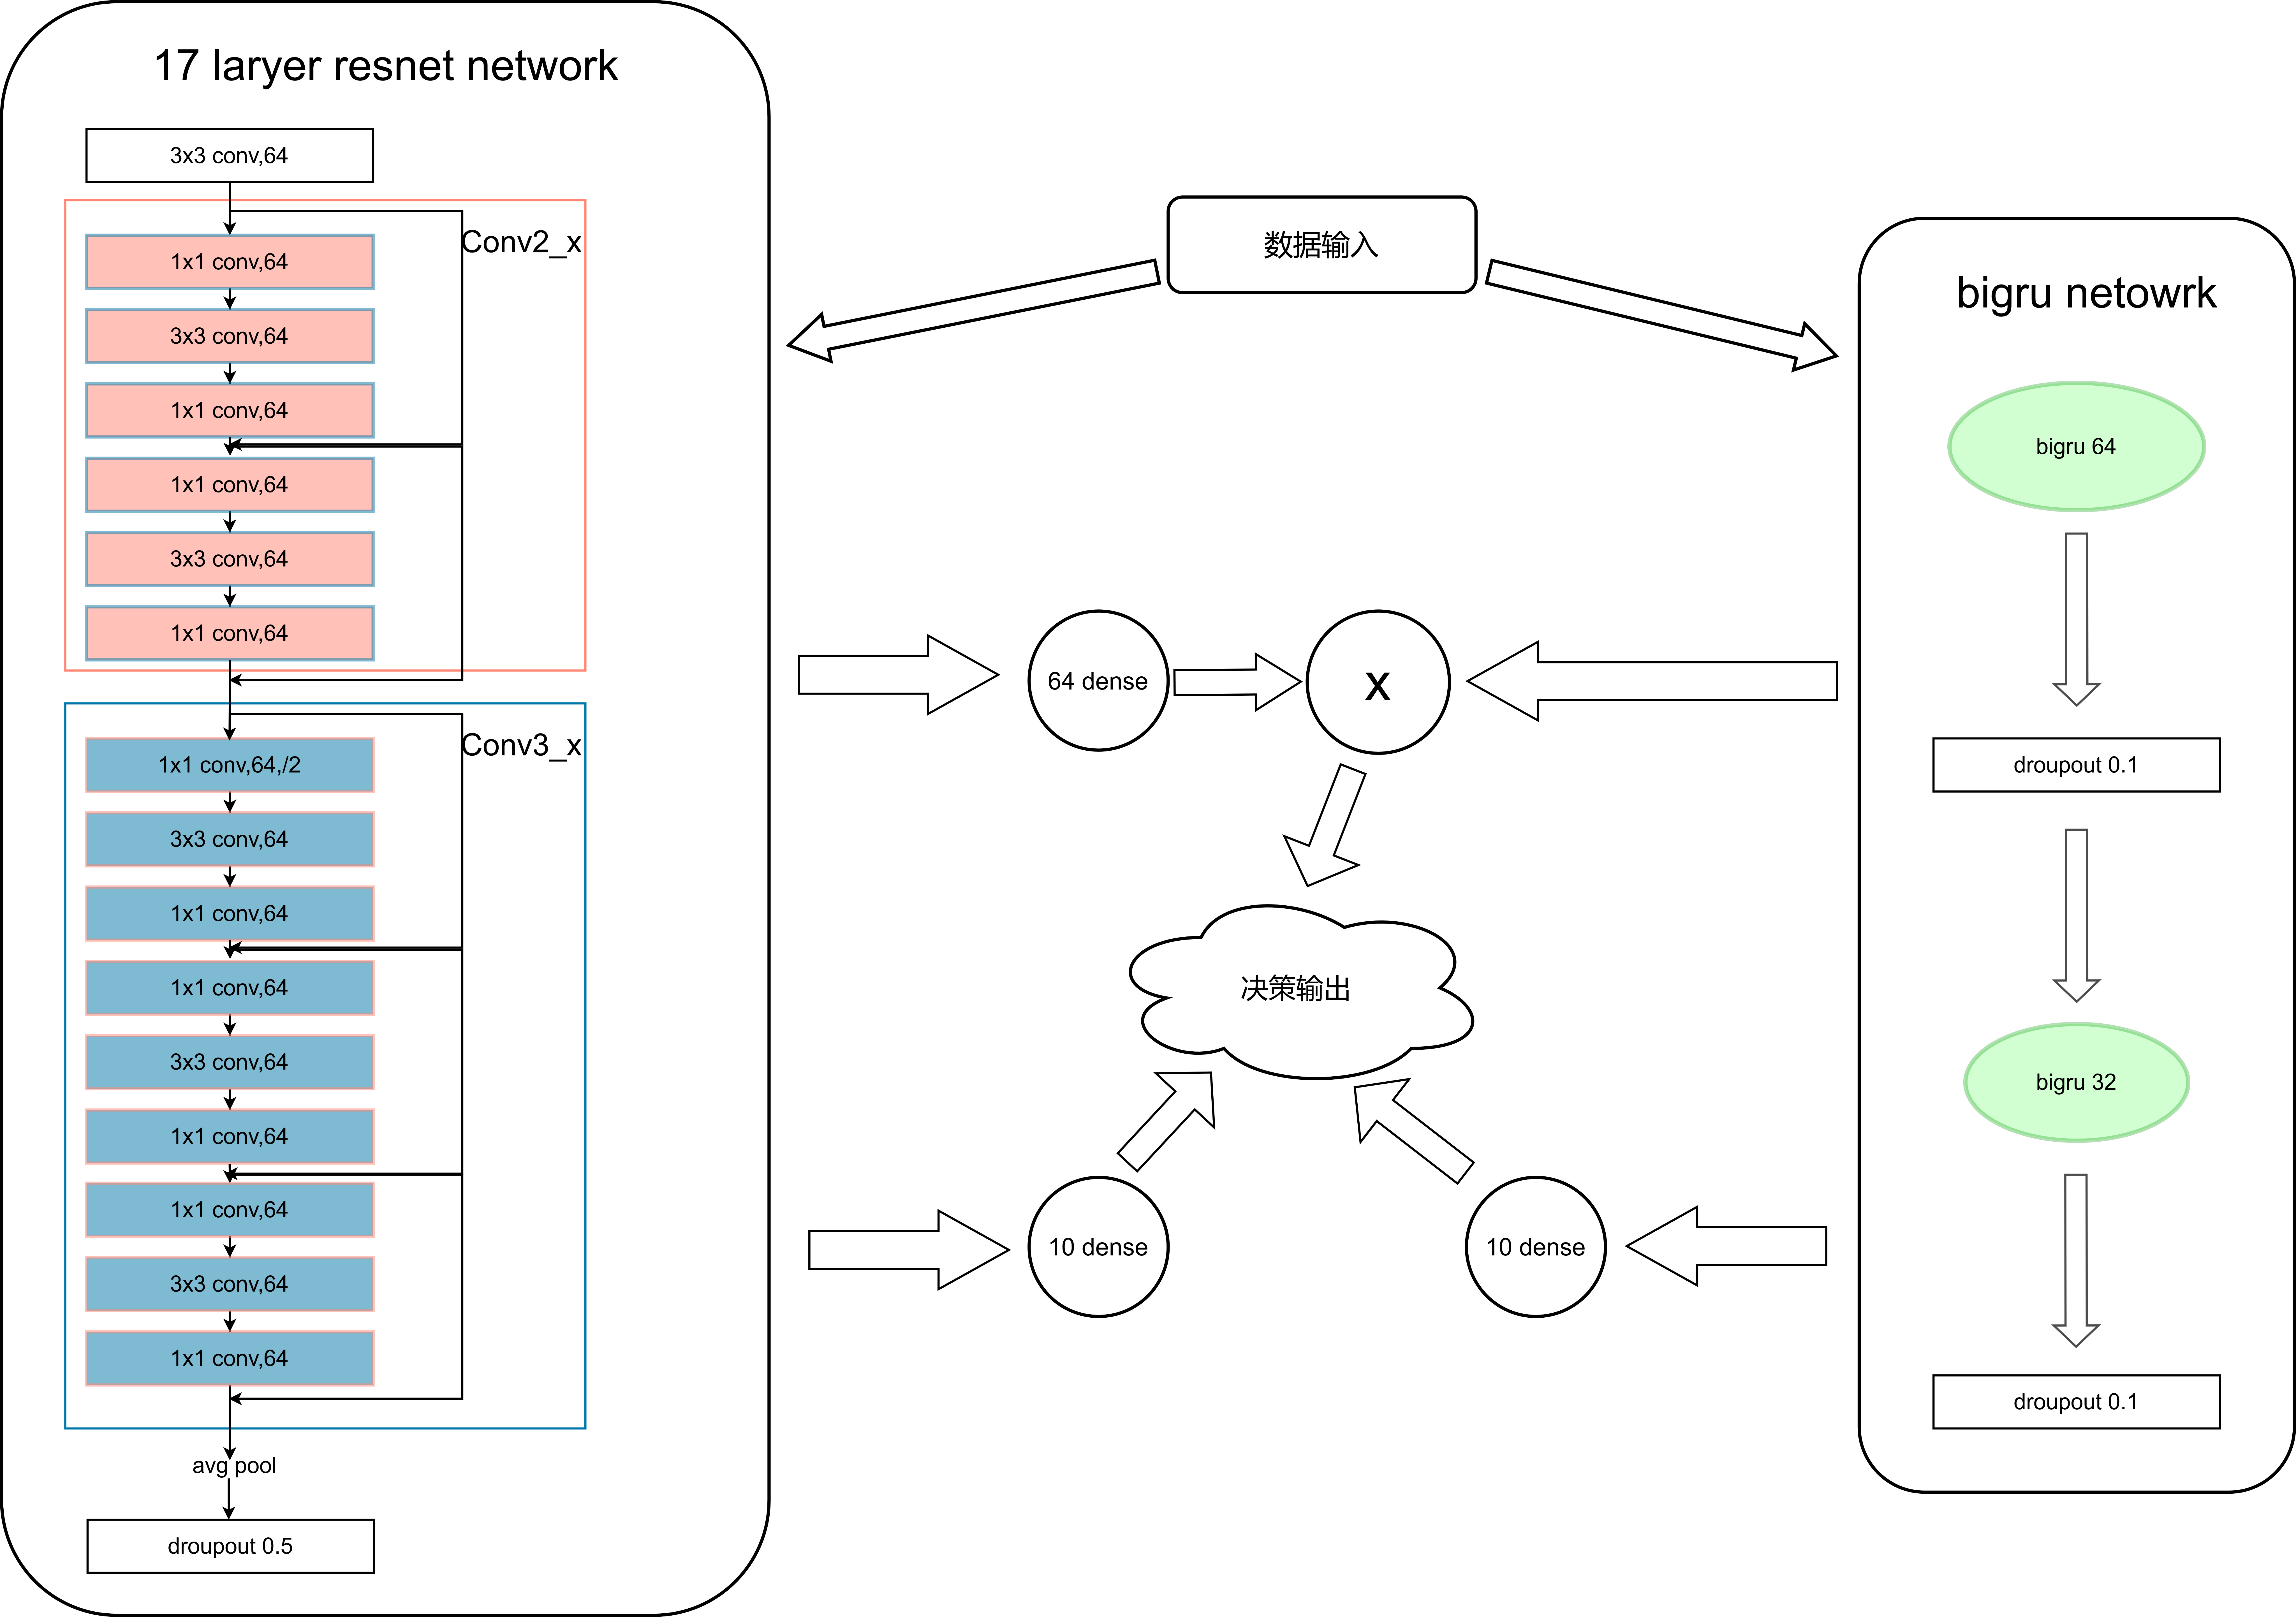
\includegraphics[width = \textwidth]{hyber_model_struction.drawio.png}
	\caption{混合模型整体结构}
	\label{fig:hyber_model_struct}
\end{figure}



\begin{table}[h]
	\caption{混合模型参数数量}
	\label{tab:model_params}
	\centering
	\begin{tabular}{ccc}
		\toprule
		\textbf{总参数} & \textbf{可训练参数数量} & \textbf{非可训练参数数量} \\
		\midrule
		1,417,510       & 1,412,518               & 4,992                     \\
		\bottomrule
	\end{tabular}
\end{table}
\subsection{数据预处理}
数据预处理是深度学习及机器学习中的关键环节,它对于构建一个干净、标准化且均衡的数据集至关重要。
预处理的主要目标是为后续的特征学习和模型训练奠定坚实的基础。
通过实施恰当的数据预处理策略,能够显著提升模型的性能、加速训练过程,并增强模型对未见数据的泛化能力。\par

以下是本文的数据预处理步骤:首先,本文对训练集和测试集进行特征编码,以确保分类数据能够被模型有效处理;
随后,本文针对原始数据集及编码过程中可能出现的缺失值进行了详尽的处理,以确保数据的完整性和准确性;
鉴于本文所使用的数据集存在显著的类别不平衡问题,本文还将对少数类样本进行过采样处理。
这一策略旨在平衡训练过程中的类别表示,从而提升模型对少数类的识别能力。
通过这一系列预处理步骤,有望构建一个更加优质的数据集,为后续的模型训练提供有力支持。\par

图~\ref{fig:dataprocess}~概括性地展示了整个数据预处理流程,本节接下来的部分将对这一流程中的关键步骤进行详细阐述。
\begin{figure}[htbp]
	\centering
	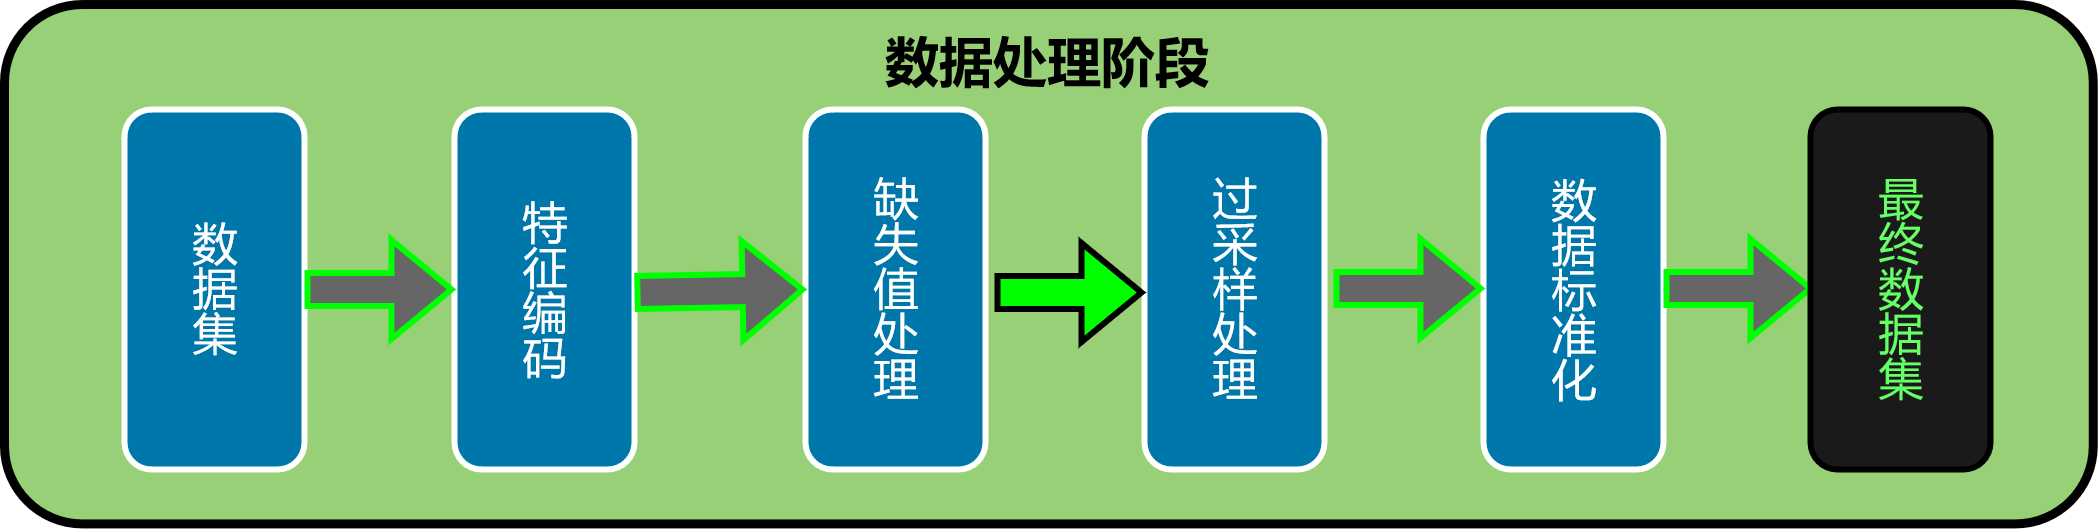
\includegraphics[width = 0.8\textwidth]{dataprocess.drawio.png}
	\caption{数据集预处理流程图}
	\label{fig:dataprocess}
\end{figure}

1)~特征编码\par

特征编码是数据预处理中不可或缺的一环,旨在将原始数据转化为模型能够识别和处理的数值格式。
这个过程对于提高模型的性能和准确性至关重要,因为大多数模型的预期输入数据为数值型,而原始数据往往包括各种类型,如文本、日期或分类数据。
特征编码目的便是将非数值特征转换为数值形式,使模型能够对这些数据进行计算。
在本文所使用的流量数据集中,同样存在大量非数值类型的特征,如IP地址、协议类型等。
为了充分利用这些数据并构建有效的模型,需要对这些非数值特征进行特征编码,将其转换为数值类型。\par

One-Hot 编码是一种特殊且广泛使用的特征编码方法,它易于理解和实现,非常适用于处理具有有限类别的分类数据。
鉴于其实施简便性,本文决定采用One-Hot 编码方式,针对数据集中的非数值类型特征进行转换。
该方法的工作原理是为每个类别创建一个独立的二进制列,这样每个数据点在其所属类别的对应列上被标记为1,而在其他所有列上则被标记为0。
这种方式能够有效地将非数值类型特征转换为机器学习算法易于处理的数值形式,从而提升模型的性能。
表~\ref{tab:onehot}~是这一方法的具体算法。\par
\begin{table}[htbp]
	\caption{One-hot编码算法实现}
	\label{tab:onehot}
	\centering
	\begin{tabularx}{1.0\textwidth}{cl}
		\toprule
		\multicolumn{2}{l}{\textbf{one-hot编码算法}}                              \\
		\midrule
		\multicolumn{2}{l}{\textbf{输入}: 数据集 $D$,其中包含数值型和分类型列}   \\
		\multicolumn{2}{l}{\textbf{输出}: 经过One-hot编码的数据集 $D'$}           \\
		1  & 初始化一个空的数据集 $D'$                                            \\
		2  & \textbf{for} 每一列 $col$ \textbf{in} $D$:                           \\
		3  & \quad \textbf{if} $col$ 是分类型:                                    \\
		4  & \quad\quad $unique\_values$ = 获取 $col$ 的所有唯一值                \\
		5  & \quad\quad \textbf{for} 每一个值 $val$ \textbf{in} $unique\_values$: \\
		6  & \quad\quad\quad 创建一个新列 $new\_col$,名称为 ``$col\_val$''       \\
		7  & \quad\quad\quad \textbf{for} 每一行 $row$ \textbf{in} $D$:           \\
		8  & \quad\quad\quad\quad \textbf{if} $row[col] == val$:                  \\
		9  & \quad\quad\quad\quad\quad 在 $D'[new\_col]$ 中填充 1                 \\
		10 & \quad\quad\quad\quad \textbf{else}:                                  \\
		11 & \quad\quad\quad\quad\quad 在 $D'[new\_col]$ 中填充 0                 \\
		12 & \quad \textbf{else}:                                                 \\
		13 & \quad\quad 将 $col$ 直接复制到 $D'$ 中                               \\
		14 & \textbf{return} $D'$                                                 \\
		\bottomrule
	\end{tabularx}
\end{table}

在处理IP地址时,直接进行One-Hot编码会破坏其内在特征并导致维度爆炸,影响模型性能。
常见的处理方法包括字段分割、整数转换、地理定位和嵌入法。字段分割法将IPv4地址拆分为四个数值特征,保留模式识别能力。
整数转换法将IP转为32位整数(IPv6为更大整数),保持层次结构,适合数值特征处理。
地理定位将IP映射到地理特征,如国家、城市,利用外部服务获取,适用于地域分析。
嵌入法通过深度学习将IP转换为向量,捕获地址间相似性,但计算成本高。
考虑到整数法可能引起特征不平衡,地理定位操作复杂,嵌入法计算代价大,本文采用字段分割法简化处理流程。\par

2)~数据集平衡处理\par
在大规模数据集预处理中,解决数据不平衡问题是提高模型性能和泛化能力的关键步骤。
由于本文采用的数据集是非常不均衡的,本文将会对数据集进行平衡处理。
数据不平衡通常通过欠采样和过采样两种重采样策略来处理。
欠采样通过减少多数类样本来达到平衡,虽然助于增强模型对少数类的关注,但会造成信息丢失。
相反,过采样则通过增加少数类样本数量来平衡数据,例如可以采用复制样本或利用SMOTE等高级技术生成新样本,提高少数类的代表性。\par

SMOTE(Synthetic Minority Over-sampling Technique)是一种过采样策略,通过合成新的少数类样本而非简单重复现有样本来平衡数据集。
其核心优势在于增加数据多样性,促进模型学习复杂决策边界,显著提升分类器对少数类的识别能力,改善模型性能和泛化能力。
在样本量不足时,过采样尤为适用,鉴于此,本文将会利用SMOTE算法对数据集进行平衡处理,以期提升模型的分类效果。
表~\ref{tab:smote}~是该技术的算法实现。
\begin{table}[htbp]
	\caption{SMOTE算法实现}
	\label{tab:smote}
	\centering
	\begin{tabularx}{1.0\textwidth}{cl}
		\toprule
		\multicolumn{2}{l}{\textbf{SMOTE算法}}                                              \\
		\midrule
		\multicolumn{2}{l}{\textbf{输入}: 少数类样本集 $S$,采样倍率 $N$,最近邻数 $k$}     \\
		\multicolumn{2}{l}{\textbf{输出}: 合成样本集 $S'$}                                  \\
		1  & 如果 $N$ 不是整数,则将 $N$ 向下取整,同时调整最终的样本数量                   \\
		2  & 初始化空的合成样本集 $S'$                                                      \\
		3  & \textbf{for} 每一个样本 $s$ \textbf{in} $S$:                                   \\
		4  & \quad 找到 $s$ 的 $k$ 个最近邻                                                 \\
		5  & \quad \textbf{for} $i$ \textbf{from} 1 \textbf{to} $N$:                        \\
		6  & \quad\quad 随机选择一个最近邻 $nn$                                             \\
		7  & \quad\quad \textbf{for} 每个特征 $f$:                                          \\
		8  & \quad\quad\quad 计算 $s$ 和 $nn$ 在特征 $f$ 上的差值 $\Delta f$                \\
		9  & \quad\quad\quad 生成新值 $new\_f = s[f] + \Delta f \times \text{随机数}(0, 1)$ \\
		10 & \quad\quad 创建新样本 $new\_s[i]$,其特征值为所有生成的 $new\_f$               \\
		11 & \quad\quad 将 $new\_s[i]$ 添加到合成样本集 $S'$                                \\
		12 & \textbf{return} $S'$                                                           \\
		\bottomrule
	\end{tabularx}
\end{table}
\subsection{实验评估}
\textbf{1.数据集介绍}\par
UNSW-NB15数据集\cite{moustafa2015comprehensive}由澳大利亚新南威尔士大学的网络安全实验室开发,旨在克服以往数据集的不足并提供更实际的测试环境。
与早期的KDD Cup 99和NSL-KDD数据集相比,UNSW-NB15引入了一系列的改进和特色,以适应网络威胁检测的新要求。
这些改进体现在数据集的构成、攻击类型的多样性以及数据的实用性和代表性上。
首先,UNSW-NB15数据集通过包含更现代的攻击类型,如DoS、蠕虫、后门攻击和Fuzzers等(关于具体的数据集类别占比详见表~\ref{tab:UNSW-NB15_distribution}~和图~\ref{fig:UNSW-NB15barchart}~,攻击种类详见表~\ref{tab:UNSW-NB15_class}~)。
\begin{table}[h]
	\caption{UNSW-NB15流量分布及其描述}
	\label{tab:UNSW-NB15_distribution}
	\begin{tabularx}{\textwidth}{@{}cccX@{}}
		\toprule
		\multicolumn{1}{c}{\textbf{种类}} & \multicolumn{1}{c}{\textbf{数量}} & \multicolumn{1}{c}{\textbf{占比(\%)}} & \multicolumn{1}{c}{\textbf{描述}}                                                                \\
		\midrule
		Normal                            & 2218761                           & 87.35\%                                 & 正常数据                                                                                         \\

		Fuzzers                           & 24246                             & 0.95\%                                  & 通过向程序或网络输入随机数据尝试使其悬挂或暂停的攻击                                             \\

		Analysis                          & 2677                              & 0.11\%                                  & 包含不同的端口扫描、垃圾邮件和html文件渗透攻击                                                   \\

		Backdoors                         & 2329                              & 0.09\%                                  & 一种秘密绕过系统安全机制以访问计算机或其数据的技术                                               \\

		DoS                               & 16353                             & 0.64\%                                  & 恶意尝试使服务器或网络资源对用户不可用,通常通过暂时中断或悬挂连接到互联网的主机的服务来实现     \\

		Exploits                          & 44525                             & 1.75\%                                  & 攻击者了解操作系统或软件内的安全问题,并利用这一点通过利用漏洞进行攻击                           \\

		Generic                           & 215481                            & 8.48\%                                  & 一种针对所有给定块大小和密钥大小的分组密码的技术,不考虑分组密码的结构                           \\

		Recon                             & 13987                             & 0.55\%                                  & 包含所有可以模拟收集信息攻击的攻击                                                               \\

		Shellcode                         & 1511                              & 0.06\%                                  & 利用软件漏洞进行攻击的载荷中的一小段代码                                                         \\

		Worms                             & 174                               & 0.01\%                                  & 攻击者复制自身以便传播到其他计算机,通常使用计算机网络传播,依赖于目标计算机上的安全漏洞进行传播 \\
		\bottomrule
	\end{tabularx}
\end{table}
这种多样化的攻击样本集合使得数据集不仅能够用于传统的入侵检测研究,也适用于评估面对新型攻击行为的检测系统的效果。
\begin{figure}[h]
	\centering
	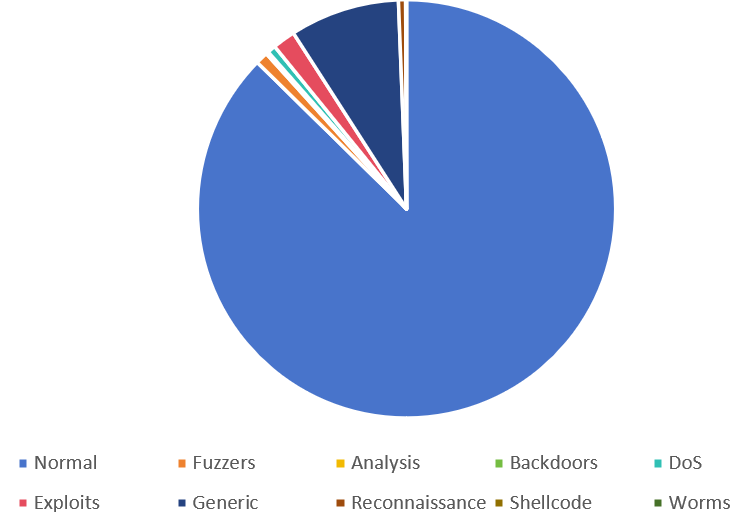
\includegraphics[width = 0.8\textwidth]{UNSW-NB15barchart.png}
	\caption{UNSW-NB15数据集分布占比饼状图}
	\label{fig:UNSW-NB15barchart}
\end{figure}

\begin{table}[htbp]
	\caption{UNSW-NB15数据集中每种攻击的不同子类的细分}
	\label{tab:UNSW-NB15_class}
	\begin{tabularx}{\textwidth}{@{}ccX@{}}
		\toprule
		\multicolumn{1}{c}{\textbf{种类}} & \multicolumn{1}{c}{\textbf{数量}} & \multicolumn{1}{c}{\textbf{子类}}                                                                                                                                                                                                                                                                                                                                                                                                                                                                                                                                   \\
		\midrule
		Fuzzers                           & 10                                & FTP, HTTP, RIP, SMB, Syslog, PPTP, TFTP, DCERPC, OSPF, BGP                                                                                                                                                                                                                                                                                                                                                                                                                                                                                                          \\
		Probe                             & 13                                & Telnet, SNMP, SunRPC Portmapper (TCP) UDP Service, SunRPC Portmapper (TCP) TCP Service, SunRPC Portmapper (UDP) UDP Service, NetBIOS, DNS, HTTP,
		SunRPC Portmapper (UDP), ICMP, SCTP, MSSQL, SMTP                                                                                                                                                                                                                                                                                                                                                                                                                                                                                                                                                                                            \\
		Shellcode                         & 15                                & FreeBSD, HP-UX, NetBSD, AIX, SCO Unix, Linux, Decoders, IRIX, OpenBSD, Mac OS X, BSD, Windows, BSDi, Multiple OS, Solaris                                                                                                                                                                                                                                                                                                                                                                                                                                           \\
		Analysis                          & 3                                 & HTML, Port Scanner, Spam                                                                                                                                                                                                                                                                                                                                                                                                                                                                                                                                            \\
		Backdoors                         & 1                                 & Backdoors                                                                                                                                                                                                                                                                                                                                                                                                                                                                                                                                                           \\
		DoS                               & 36                                & Ethernet, SunRPC, LDAP, Browser, DCERPC, Telnet, NetBIOS/SMB, DNS, TCP, Common Unix Print System (CUPS), Miscellaneous, ISAKMP, Hypervisor,
		Cisco Skinny, IIS Web Server, IGMP, ICMP, XINETD, SIP, RTSP, Windows Explorer, IRC, NTP, CUPS, Asterisk, HTTP, Microsoft Office, SSL, IMAP, SMTP, Oracle, RDP, VNC, FTP, TFTP, SNMP                                                                                                                                                                                                                                                                                                                                                                                                                                                         \\
		Exploits                          & 54                                & Clientside Microsoft Paint, Dameware, Clientside Microsoft Media Player, SSH, SCCP, Unix r Service, SunRPC, LDAP, Web Application, Browser, DCERPC, Interbase, Telnet, DNS, TCP, Webserver, SCADA, SMB, Miscellaneous, Cisco IOS, All, LPD, RADIUS, RDesktop, Unix 'r' Service, IGMP, POP3, ICMP, Clientside Microsoft, Microsoft IIS, Backup Appliance, IDS, Apache, NNTP, RTSP, Evasions, SIP, WINS, Office Document, PHP, Clientside Microsoft Office, Miscellaneous Batch, Browser FTP, MSSQL, SOCKS, PPTP, Clientside, SSL, IMAP, SMTP, Oracle, VNC, FTP, TFTP \\
		Generic                           & 7                                 & All,SIP,HTTP,SMTP,IXIA,TFTP,Superflow                                                                                                                                                                                                                                                                                                                                                                                                                                                                                                                               \\
		Recon                             & 14                                & DNS, HTTP, ICMP, MSSQL, NetBIOS, SCTP, SMTP, SNMP, SunRPC, SunRPC Portmapper (TCP) TCP Service, SunRPC Portmapper (TCP) UDP Service, SunRPC Portmapper (UDP) TCP Service, SunRPC Portmapper (UDP) UDP Service, Telnet                                                                                                                                                                                                                                                                                                                                               \\
		Worms                             & 1                                 & Worms                                                                                                                                                                                                                                                                                                                                                                                                                                                                                                                                                               \\
		\bottomrule
	\end{tabularx}
\end{table}\par

其次,UNSW-NB15提供了四个CSV格式的数据记录文件,每个文件都包含了攻击记录和正常记录,共2,540,044条记录。
海量的数据集不仅有助于模型的训练和验证,也提高了入侵检测模型在实际环境中应用的可信度和有效性。
此外,UNSW-NB15数据集在设计时注重了实用性和代表性,通过模拟现实世界的网络环境和流量模式,确保了数据集的广泛适用性和长期价值。
这使得该数据集成为评估和比较不同入侵检测技术性能的理想选择。\par

\textbf{2.实验环境}\par
为了评估本文所提方案的有效性,本文将利用python语言来实现以上流程,并选用表~\ref{tab:env_setting}~中的配置来进行实验。
\begin{table}[htbp]
	\caption{实验设备配置}
	\label{tab:env_setting}
	\centering
	\begin{tabular}{ccc}
		\toprule
		\textbf{环境类别}         & \textbf{设备项目} & \textbf{项目参数}                  \\
		\midrule
		\multirow{6}{*}{硬件环境} & CPU型号           & Intel(R) Core(TM) i7-11800H        \\
		                          & CPU规格           & 8核16线程@2.30GHz                  \\
		                          & GPU型号           & NVIDIA GeForce RTX 3060 Laptop GPU \\
		                          & 内存大小          & 16.0 GB                            \\
		                          & 硬盘类型          & SSD                                \\
		                          & 硬盘大小          & 1TB                                \\
		\hline
		\multirow{3}{*}{软件环境} & 操作系统          & Windows 11                         \\
		                          & 开发语言          & Python 3.11.7                      \\
		                          & 编辑器            & Visual Studio Code                 \\
		\bottomrule
	\end{tabular}
\end{table}

\textbf{3.评估指标}\par
本文主要使用准确度 (Accuracy)、精确度 (Precision)、召回率 (Recall)、加权平均 F1 分数 (Macro Averaged F1 Score)、宏平均 F1 分数 (Macro Averaged F1 Score)这5个评价指标对本文的方案进行全方位的评估。
以下是这5个指标的简单介绍。\par
1)~准确度\par
表示模型正确预测的比例,即在模型进行的所有预测中,正确预测所占的比例。
\begin{equation}
	\label{eq:val_score1}
	Accuracy = \frac{Number of Correct Predictions}{Total Number of Predictions} = \frac{TP + TN}{TP + TN + FP + FN}
\end{equation}

2)~精确度\par
简称精度,也称为查准率,是所有模型预测为正类的样本中,实际为正类的比例。
\begin{equation}
	\label{eq:val_score2}
	Precision = \frac{TP}{TP + FP}
\end{equation}

3)~召回率\par
召回率,也称为真正率、查补率,是模型正确识别为正类的样本占所有实际正类样本的比例。
\begin{equation}
	\label{eq:val_score3}
	Recall = \frac{TP}{TP + FN}
\end{equation}

4)~宏平均~F1~分数\par
宏平均~F1~分数是一种性能评估指标,用于衡量模型在所有类别上的平均表现。
它通过简单地计算所有类别~F1~分数的算术平均值得出,每个类别被赋予相同的权重,不论其样本量大小。
\begin{equation}
	\label{eq:val_score4}
	F1_{macro} = \frac{1}{N} \sum\limits_{i=1}^{N} F1_i
\end{equation}
\begin{flushleft}
	\renewcommand\arraystretch{1.25}
	\begin{tabularx}{\textwidth}{@{}>{\normalsize\rm}l@{\quad}>{\normalsize\rm}l@{——}>{\normalsize\rm}X@{}}
		式中 & $F1_{macro}$ & 表示宏平均 F1 分数;          \\
		     & $N$          & 类别总数;                    \\
		     & $F1_i$       & 表示第 $i$ 个类别的 F1 分数。 \\
	\end{tabularx}\vspace{.5ex}
\end{flushleft}
宏平均 F1 分数特别适用于样本分布不均匀的数据集,因为它给每个类别分配了同等的重要性。
这样做确保了即使某些类别的样本数量很少,它们在计算平均分数时也会有相等的影响。\par

5)~加权平均 F1 分数\par
加权平均F1分数是一种性能评估指标,通过根据每个类别的样本量对其F1分数进行加权平均,以反映所有类别的整体性能。
每个类别的重要性通过其在数据集中的相对比例来确定。
\begin{equation}
	\label{eq:val_score5}
	F1_{weighted} = \sum\limits_{i=1}^{N} w_i \cdot F1_i
\end{equation}
\begin{flushleft}
	\renewcommand\arraystretch{1.25}
	\begin{tabularx}{\textwidth}{@{}>{\normalsize\rm}l@{\quad}>{\normalsize\rm}l@{——}>{\normalsize\rm}X@{}}
		式中 & $F1_{weighted}$ & 加权平均F1分数;                                                  \\
		     & $N$             & 类别总数;                                                        \\
		     & $F1_i$          & 第$i$个类别的F1分数                                               \\
		     & $w_i$           & 第$i$个类别的权重,通常由该类别的样本数量占总样本数量的比例确定。 \\
	\end{tabularx}\vspace{.5ex}
\end{flushleft}

上式\ref{eq:val_score1}、\ref{eq:val_score2}、\ref{eq:val_score3}%、\ref{eq:val_score4}、\ref{eq:val_score5}\ref{eq:val_score6}、\ref{eq:val_score7}%
中,
$TP$(True Positives)表示正确地将正类预测为正类;
$TN$(True Negatives)表示正确地将负类预测为负类;
$FP$(False Positives)表示错误地将负类预测为正类;
$FN$(False Negatives)表示错误地将正类预测为负类。

\textbf{4.特征编码效果实验评估}\par
在本次实验中,本文通过比较特征编码前后各种机器学习和深度学习模型的准确率(如表~\ref{tab:model_performance}~以及图~\ref{fig:comapre_accuracy_encoding}~所示,
\begin{figure}[htbp]
	\centering
	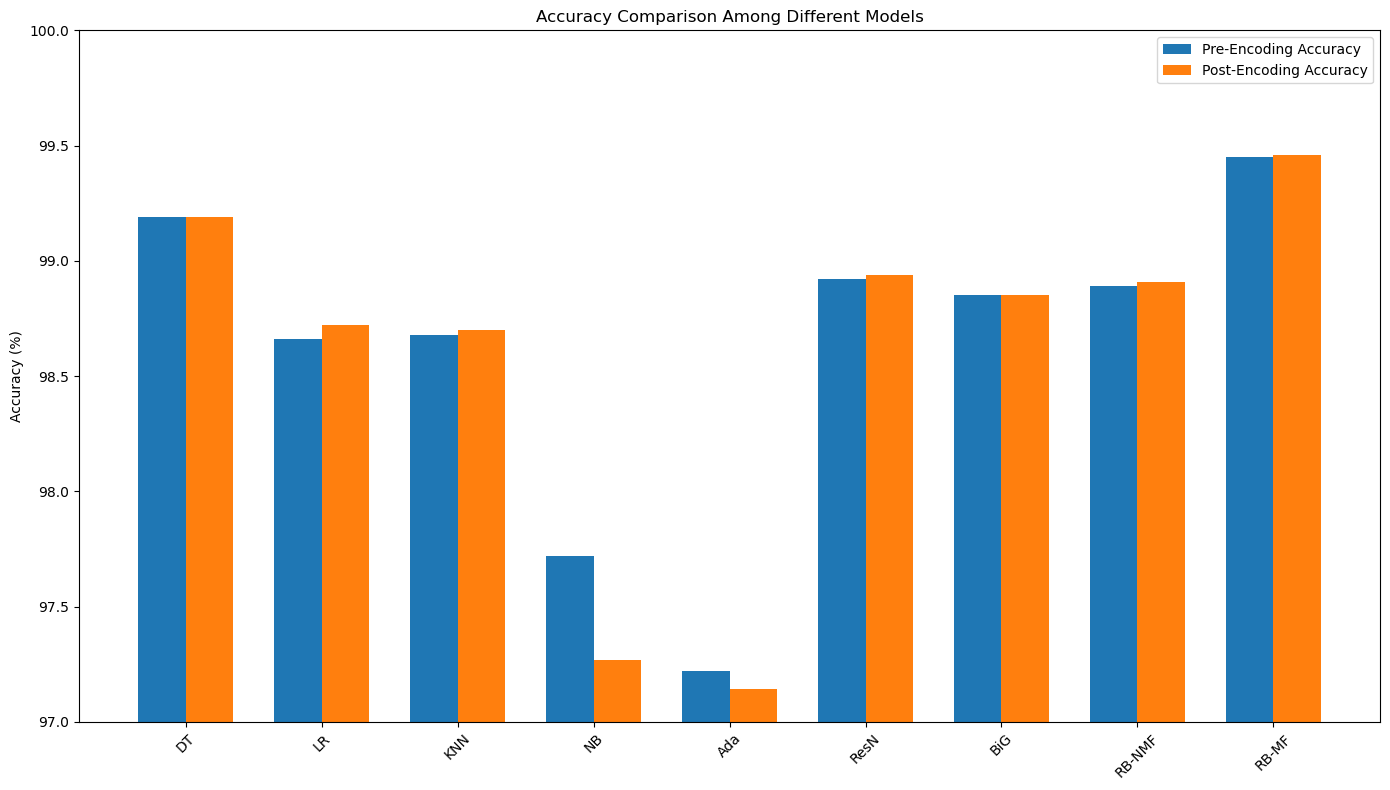
\includegraphics[width = \textwidth]{acc.png}
	\caption{特征编码前后模型预测准确率对比条状图}
	\label{fig:comapre_accuracy_encoding}
\end{figure}
\begin{table}[htbp]
	\centering
	\setlength{\tabcolsep}{1pt}
	\caption{特征编码前后模型表现}
	\label{tab:model_performance}
	\begin{tabular}{cccccccccc}
		\toprule
		        & DT               & LR              & KNN             & NB             & Ada               & ResN            & BiG           & RB-NMF          & RB-MF           \\
		\midrule
		\multicolumn{9}{c}{\textbf{特征编码前}}                                                                                                                                   \\
		Acc     & 99.19\%          & 98.66\%         & 98.68\%         & 97.72\%        & 97.22\%           & 98.92\%         & 98.85\%       & 98.89\%         & 99.45\%         \\
		f1\_mac & 0.5422           & 0.3730          & 0.4042          & 0.3376         & 0.3609            & 0.4110          & 0.493         & 0.518           & 0.529           \\
		f1\_wei & 0.9925           & 0.9874          & 0.9872          & 0.9726         & 0.9704            & 0.9892          & 0.9885        & 0.9891          & 0.9945          \\
		\midrule
		\multicolumn{9}{c}{\textbf{特征编码后}}                                                                                                                                   \\
		Acc     & 99.19\%          & 98.72\%\uparrow & 98.70\%\uparrow & 97.27\%        & 97.14\%\downarrow & 98.94\%\uparrow & 98.85\%       & 98.91\%\uparrow & 99.46\%\uparrow \\
		f1\_mac & 0.5378\downarrow & 0.3871\uparrow  & 0.4090\uparrow  & 0.2166         & 0.3197\downarrow  & 0.4166\uparrow  & 0.495\uparrow & 0.52\uparrow    & 0.53\uparrow    \\
		f1\_wei & 0.9925           & 0.9879\uparrow  & 0.9873\uparrow  & 0.9729\uparrow & 0.9723\uparrow    & 0.9898\uparrow  & 0.9885        & 0.9892\uparrow  & 0.9946\uparrow  \\
		\bottomrule
	\end{tabular}
\end{table}
其中DT、LR、KNN、 NB、 Ada、ResN、BiG、RB-NMF、RB-MF分别代表决策树、逻辑回归、K近邻、朴素贝叶斯、Ada增强、残差神经网络、双向门控循环单元、未经过多模态特征融合的残差神经网络与门控循环单元混合模型以及经过多模态特征融合的残差神经网络与门控循环单元混合模型),得出了一些发现。
首先,决策树模型在应对输入数据表示形式的变化时,表现出卓越的鲁棒性,其准确率在特征编码前后基本保持不变。
相比之下,逻辑回归和K近邻等模型在特征编码后轻微提升了准确率,这表明特征编码可能会对这些模型带来微小的性能提升。
然而,朴素贝叶斯模型在特征编码后的准确率却出现显著的下降。
这主要是由于特征编码改变了数据的原始分布假设,从而对基于概率的朴素贝叶斯模型产生较大的影响。
在深度学习领域,ResNet和BiGRU模型在特征编码后准确率则得到稳定提升。
这主要归功于这些模型能够从编码后的特征中学习到更为复杂和深层的数据表示。
特别值得一提的是,采用多模态特征融合的ResNet-BiGRU模型在特征编码前后准确率均最高。
尤其在特征编码后,其准确率更是高达99.46\%,这充分凸显了模态融合在提升模型处理能力方面的显著优势。\par


整体而言,所有模型在准确率方面都表现出较高的水平,特别是在特征编码后,大多数模型的准确率略有提升,说明特征编码对模型性能有正面影响。
具体到F1分数,F1 Macro(图~\ref{fig:f1_macro_score}~)和F1 Weighted(图~\ref{fig:f1_weighted_score}~)分数在特征编码后也显示出类似的趋势。
\begin{figure}[htbp]
	\centering
	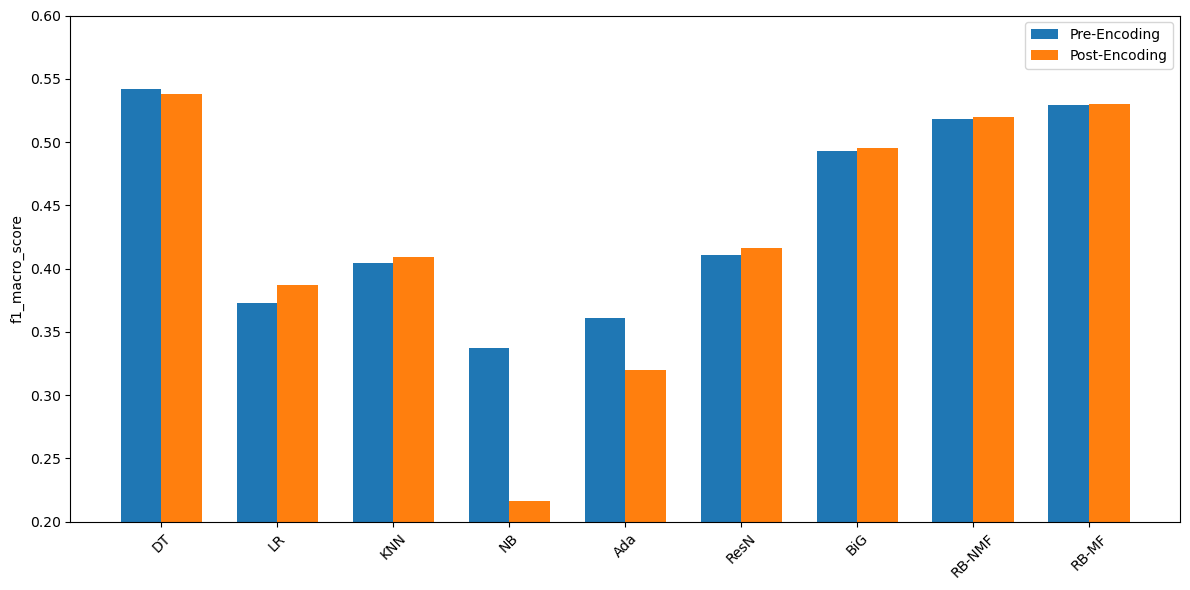
\includegraphics[width = \textwidth]{f1-mac.png}
	\caption{特征编码前后模型f1 macro score对比条状图}
	\label{fig:f1_macro_score}
\end{figure}
\begin{figure}[htbp]
	\centering
	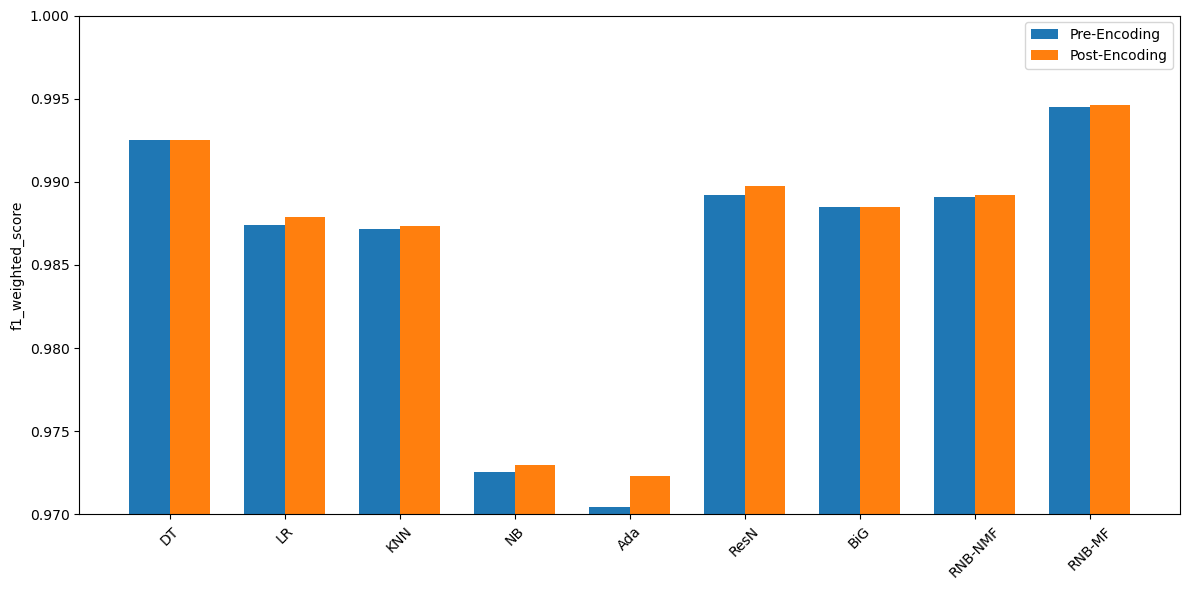
\includegraphics[width = \textwidth]{f1-wei.png}
	\caption{特征编码前后模型f1 weighted score对比条状图}
	\label{fig:f1_weighted_score}
\end{figure}
在深度学习模型方面,ResNet和BiGRU表现出了较好的性能提升,尤其是在特征编码后,这主要归因于深度学习模型能够从编码后的特征中学习到更加复杂的表示。
同样值得注意的是,采用模态融合策略的ResNet-BiGRU模型在所有评价指标上都表现最优,无论是在特征编码前还是编码后。
经过对数据的细致分析后,可以看到特征编码和模型选择对于提升模型性能具有重要意义。
模态特征融合技术尤其在提高复杂模型的准确率和F1分数方面显示出显著的优势,这为未来模型设计和特征工程方面的研究提供了有价值的参考。\par

\textbf{5.数据集平衡处理效果实验评估}\par
处理网络流量数据时,一个普遍面临的挑战是数据的不均衡性,特别是在网络安全领域尤为突出,因为正常流量的样本数量远超过异常流量或攻击流量的样本数量。
例如,在本章所使用的数据集中,正常流量样本占据了总样本的87\%,因此,即使模型简单地将所有流量都判断为正常流量,其准确率依然能够达到87\%。
然而,这种“一刀切”的模型在异常流量检测任务中毫无效果,因为它无法识别出任何异常样本。\par

为了解决这一问题,本文将采用SMOTE算法对异常样本进行过采样处理。
这种方法能够增加异常流量样本的数量,从而改善训练数据的平衡性。
过采样的结果如表~\ref{tab:attack_num_transposed_part1}~所示,
\begin{table}[h]
	\centering
	\caption{数据集平衡处理前后数据量变化}
	\label{tab:attack_num_transposed_part1}
	\begin{tabular}{cccccc}
		\toprule
		攻击种类          & \textbf{Fuzzers} & \textbf{Analysis} & \textbf{Backdoors} & \textbf{DoS} & \textbf{Exploits} \\
		\midrule
		\textbf{过采样前} & 3775             & 382               & 400                & 879          & 4038              \\
		\textbf{过采样后} & 50844            & 50844             & 50844              & 50844        & 50844             \\
		\bottomrule
	\end{tabular}
	\begin{tabular}{ccccc}
		\toprule
		攻击种类          & \textbf{Generic} & \textbf{Recon} & \textbf{Shellcode} & \textbf{Worms} \\
		\midrule
		\textbf{过采样前} & 5587             & 1316           & 164                & 18             \\
		\textbf{过采样后} & 50844            & 50844          & 50844              & 50844          \\
		\bottomrule
	\end{tabular}
\end{table}
从中可以看出,过采样后各类样本的数量有了明显的变化。
此外,本文使用PCA(主成分分析)方法将样本降维到了2D平面上,并在图~\ref{fig:prepostsmote}中展示了过采样前后的情况。
\begin{figure}[htbp]
	\centering
	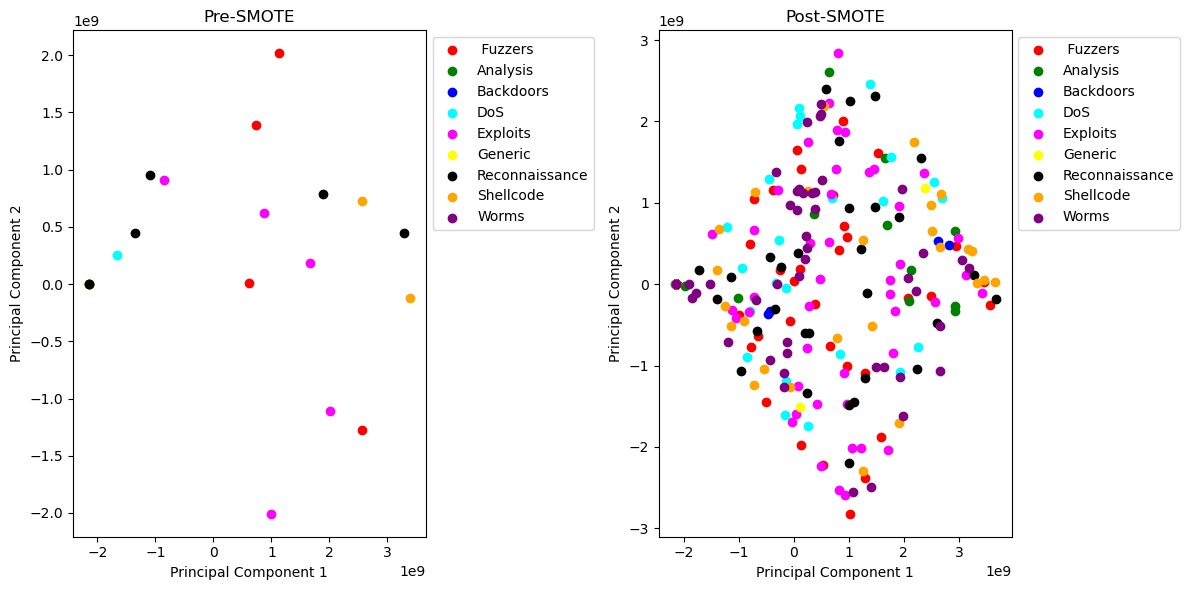
\includegraphics[width = 0.8 \textwidth]{smote.png}
	\caption{SMOTE过采样前后,1,000个样本中各种攻击类别的样本点变化,这里省略了normal样本点}
	\label{fig:prepostsmote}
\end{figure}
从图中可以看到,攻击样本的数量在过采样后有了显著的增加,这有助于模型学习到更加均衡的数据表示。\par

最终,本文评估了过采样对模型性能的影响。
表~\ref{tab:model_performance_oversampling}~展示了过采样前后各类样本检测的召回率变化。
\begin{table}[htbp]
	\centering
	\caption{过采样前后各种攻击检测召回率变化}
	\label{tab:model_performance_oversampling}
	\begin{tabular}{cccccccccc}
		\toprule
		          & DT    & LR    & KNN   & NB    & Ada   & ResN  & BiG   & RB-NMF & RB-MF \\
		\midrule
		\multicolumn{10}{c}{\textbf{过采样前}}                                             \\
		Fuzzers   & 0.825 & 0.624 & 0.614 & 0.019 & 0.064 & 0.713 & 0.709 & 0.699  & 0.842 \\
		Analysis  & 0.115 & 0     & 0     & 0.566 & 0.844 & 0     & 0     & 0      & 0.361 \\
		Backdoors & 0     & 0     & 0     & 0     & 0.059 & 0     & 0     & 0      & 0.288 \\
		DoS       & 0.165 & 0.051 & 0.114 & 0.008 & 0     & 0.017 & 0.322 & 0.341  & 0.458 \\
		Exploits  & 0.666 & 0.705 & 0.639 & 0.04  & 0.001 & 0.808 & 0.716 & 0.796  & 0.796 \\
		Generic   & 0.962 & 0.925 & 0.931 & 0.956 & 0.921 & 0.935 & 0.876 & 0.899  & 0.943 \\
		Recon     & 0.91  & 0.755 & 0.58  & 0.019 & 0.854 & 0.739 & 0.743 & 0.757  & 0.946 \\
		Shellcode & 0.66  & 0     & 0.14  & 0.98  & 0.76  & 0.067 & 0.045 & 0.073  & 0.937 \\
		Worms     & 0     & 0     & 0     & 0.75  & 0     & 0     & 0     & 0      & 0     \\
		normal    & 1     & 0.997 & 0.997 & 0.993 & 0.99  & 0.998 & 0.999 & 0.999  & 0.999 \\
		\midrule
		\multicolumn{10}{c}{\textbf{过采样后}}                                             \\
		Fuzzers   & 0.838 & 0.041 & 0.701 & 0.099 & 0.606 & 0.723 & 0.714 & 0.703  & 0.857 \\
		Analysis  & 0.452 & 0.032 & 0.565 & 0     & 0     & 0.013 & 0     & 0      & 0.564 \\
		Backdoors & 0.362 & 0.31  & 0.431 & 0.931 & 0.948 & 0     & 0     & 0      & 0.412 \\
		DoS       & 0.521 & 0     & 0.479 & 0.009 & 0     & 0.023 & 0.125 & 0.16   & 0.634 \\
		Exploits  & 0.807 & 0     & 0.659 & 0.026 & 0     & 0.809 & 0.714 & 0.806  & 0.822 \\
		Generic   & 0.992 & 0.187 & 0.948 & 0     & 0.926 & 0.941 & 0.875 & 0.893  & 0.941 \\
		Recon     & 0.995 & 0     & 0.872 & 0.511 & 0     & 0.724 & 0.742 & 0.759  & 0.933 \\
		Shellcode & 1     & 0     & 0.933 & 0.133 & 0.867 & 0.132 & 0.044 & 0.081  & 0.961 \\
		Worms     & 1     & 0     & 1     & 0     & 1     & 0     & 0     & 0      & 0     \\
		normal    & 1     & 0.99  & 0.97  & 0.624 & 0.985 & 0.996 & 0.999 & 0.999  & 0.999 \\
		\bottomrule
	\end{tabular}
\end{table}
通过分析该表格可知,过采样后,绝大多数模型在检测各类攻击事件时的召回率有了一定提高。
尤其是对于那些原本难以被检测到的攻击类型,如Backdoors、Analysis等,过采样为这些攻击类型提供了更多的样本,使得模型能够学习到更加丰富的特征,从而在这些攻击类型上获得了更好的召回率。\par

表~\ref{tab:oversampling_performance}~则展示了过采样前后各类样本检测精确度的变化。
\begin{table}[htbp]
	\centering
	\caption{过采样前后各种攻击检测精度变化}
	\label{tab:oversampling_performance}
	\begin{tabular}{lccccccccc}
		\toprule
		          & DT    & LR    & KNN   & NB    & Ada   & ResN  & BiG   & RB-NMF & RB-MF \\
		\midrule
		\multicolumn{10}{c}{\textbf{过采样前}}                                             \\
		Fuzzers   & 0.659 & 0.455 & 0.497 & 0.667 & 0.545 & 0.542 & 0.534 & 0.536  & 0.697 \\
		Analysis  & 1     & 0     & 0     & 0.117 & 0.054 & 0     & 0     & 0      & 0.201 \\
		Backdoors & 0.0   & 0.0   & 0     & 0     & 0.092 & 0     & 0     & 0      & 0     \\
		DoS       & 0.255 & 0.279 & 0.206 & 0.222 & 0.0   & 0.250 & 0.23  & 0.17   & 0.27  \\
		Exploits  & 0.662 & 0.623 & 0.649 & 0.763 & 0.200 & 0.620 & 0.411 & 0.656  & 0.686 \\
		Generic   & 0.966 & 0.988 & 0.983 & 0.589 & 0.997 & 0.966 & 0.746 & 0.826  & 0.979 \\
		Recon     & 0.894 & 0.562 & 0.567 & 0.019 & 0.320 & 0.747 & 0.743 & 0.863  & 0.905 \\
		Shellcode & 0.767 & 0.0   & 0.538 & 0.04  & 0.365 & 1     & 0.665 & 0.665  & 0.732 \\
		Worms     & 0.0   & 0     & 0     & 0.009 & 0     & 0     & 0     & 0      & 0     \\
		normal    & 1     & 0.998 & 0.997 & 0.998 & 0.99  & 0.998 & 0.999 & 0.999  & 0.999 \\
		\midrule
		\multicolumn{10}{c}{\textbf{过采样后}}                                             \\
		Fuzzers   & 0.756 & 0.22  & 0.409 & 0.427 & 0.465 & 0.566 & 0.512 & 0.536  & 0.772 \\
		Analysis  & 0.065 & 0.037 & 0.147 & 0     & 0     & 0.052 & 0     & 0      & 0.253 \\
		Backdoors & 0.053 & 0.032 & 0.135 & 0.011 & 0.140 & 0.013 & 0.112 & 0      & 0     \\
		DoS       & 0.17  & 0     & 0.162 & 0.002 & 0     & 0.102 & 0.24  & 0.205  & 0.24  \\
		Exploits  & 0.762 & 0     & 0.458 & 0.412 & 0     & 0.505 & 0.311 & 0.493  & 0.801 \\
		Generic   & 0.973 & 0.274 & 0.972 & 0     & 0.996 & 0.921 & 0.446 & 0.801  & 0.978 \\
		Recon     & 0.889 & 0     & 0.333 & 0.007 & 0     & 0.355 & 0.636 & 0.799  & 0.884 \\
		Shellcode & 0.793 & 0     & 0.108 & 0.035 & 0.28  & 0.204 & 0.541 & 0.637  & 0.774 \\
		Worms     & 0     & 0     & 0.004 & 0     & 0.002 & 0     & 0     & 0      & 0     \\
		normal    & 0.999 & 0.976 & 0.999 & 0.999 & 0.995 & 0.996 & 0.999 & 0.999  & 0.999 \\
		\bottomrule
	\end{tabular}
\end{table}
在检测精度方面,过采样后由于引入了更多的少数类样本导致某些模型在个别攻击类型上的精度有所下降,
% 为了提高对这些少数类的识别准确率,模型可能会在一定程度上牺牲对多数类的识别精度。
然而,从整体上看,模型的总体性能是得到了改善的。\par

另外,RB-MF(表中的RB-MF),即经过模态融合的残差网络和双向门控循环单元的混合模型,表现出了卓越的性能。
过采样后,几乎所有攻击类型的召回率均有所提高,同时精度在大多数情况下也得以保持甚至略有提升。
这说明RB-MF模型能够有效利用过采样带来的额外信息,而且模态融合策略提高了模型处理不平衡数据的能力,使其在面对复杂的攻击检测任务时,能够更加准确地识别出少数类攻击样本,同时保持对正常流量的高识别精度。\par


图~\ref{fig:ResNet-BiGRU-NoFusion-loss}~、~\ref{fig:ResNet-BiGRU-Fusion-loss}~分别是RB-NMF以及RB-MF各epoch的损失曲线以及准确率曲线。
\begin{figure}[htbp]
	\centering
	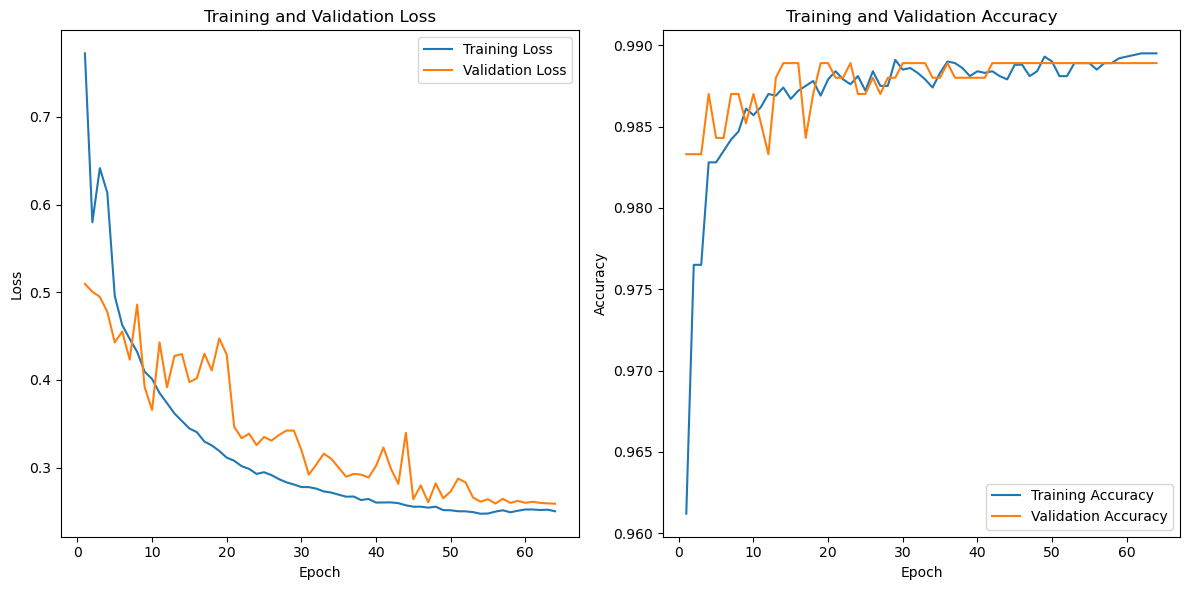
\includegraphics[width = \textwidth]{resnet_bigure_nmf.png}
	\caption{RB-NMF各epoch的损失曲线以及准确率曲线}
	\label{fig:ResNet-BiGRU-NoFusion-loss}
\end{figure}
\begin{figure}[htbp]
	\centering
	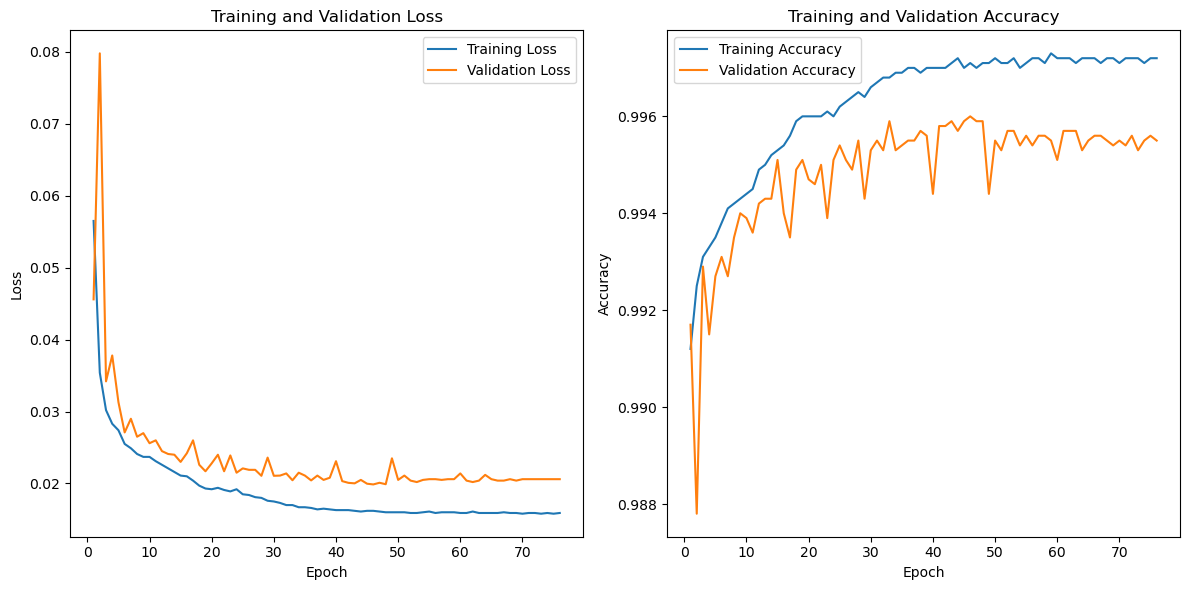
\includegraphics[width = \textwidth]{resnet_bigure_curve.png}
	\caption{RB-MF各epoch的损失曲线以及准确率曲线}
	\label{fig:ResNet-BiGRU-Fusion-loss}
\end{figure}
通过观察损失函数图表可知,未经模态融合的模型训练和验证损失都在逐渐减小,但验证损失的波动较大,这可能表明模型在训练集上有过拟合的趋势。
相比之下,经过模态融合的模型损失下降更为平滑,且在训练后期,验证损失几乎与训练损失保持一致,这表明模型具有更好的泛化能力。\par
虽然未经模态融合的模型在初期展现出了相对较高的准确率,但在训练过程中,其性能出现了明显的波动,特别是在验证准确率方面,出现这一现象的原因极有可能是模型存在过拟合问题。
相比之下,经过模态融合的模型不仅在训练初期就迅速提升了准确率,而且在后续的训练过程中也持续保持在非常高的水平,几乎没有任何波动。
这一结果充分体现了本文所设计的模型强大的稳定性和预测准确率。\par

\section{基于特征融合模型的增量学习方案}
在前几个小节中,本文已经通过实验验证了RB-MF模型在网络攻击检测任务上的性能优势。
具体而言,此模型针对UNSW-NB15数据集中的网络流量数据展现出了卓越的处理效果。
然而,值得注意的是,该模型的应用范围会受到其训练数据集独特性质的制约。
这意味着,当面对与UNSW-NB15数据集具有显著不同的新数据时,模型的表现可能会受到一定的影响。
例如,随着时间推移,新数据的不断累积使得模型需不断适应新增的信息,而旧数据可能因存储限制或隐私保护政策等因素而逐渐失去可用性。
此外,学习任务的复杂度亦可能随之增加,如分类任务中类别数的增长等,而这些变化往往无法事先预定义。\par

因此,探索如何有效地使模型适应新类型的数据,以及如何在数据动态变化的情境下保持模型的稳定性和准确性,成为了重要的研究课题。
针对这一问题,增量学习(Incremental Learning)的概念便成为解决上述问题的一个有效途径。
增量学习(图~\ref{fig:incremental_learning}~所示)旨在使模型能够逐渐适应新数据或新任务,而无需从头开始重新训练模型。
\begin{figure}[htbp]
	\centering
	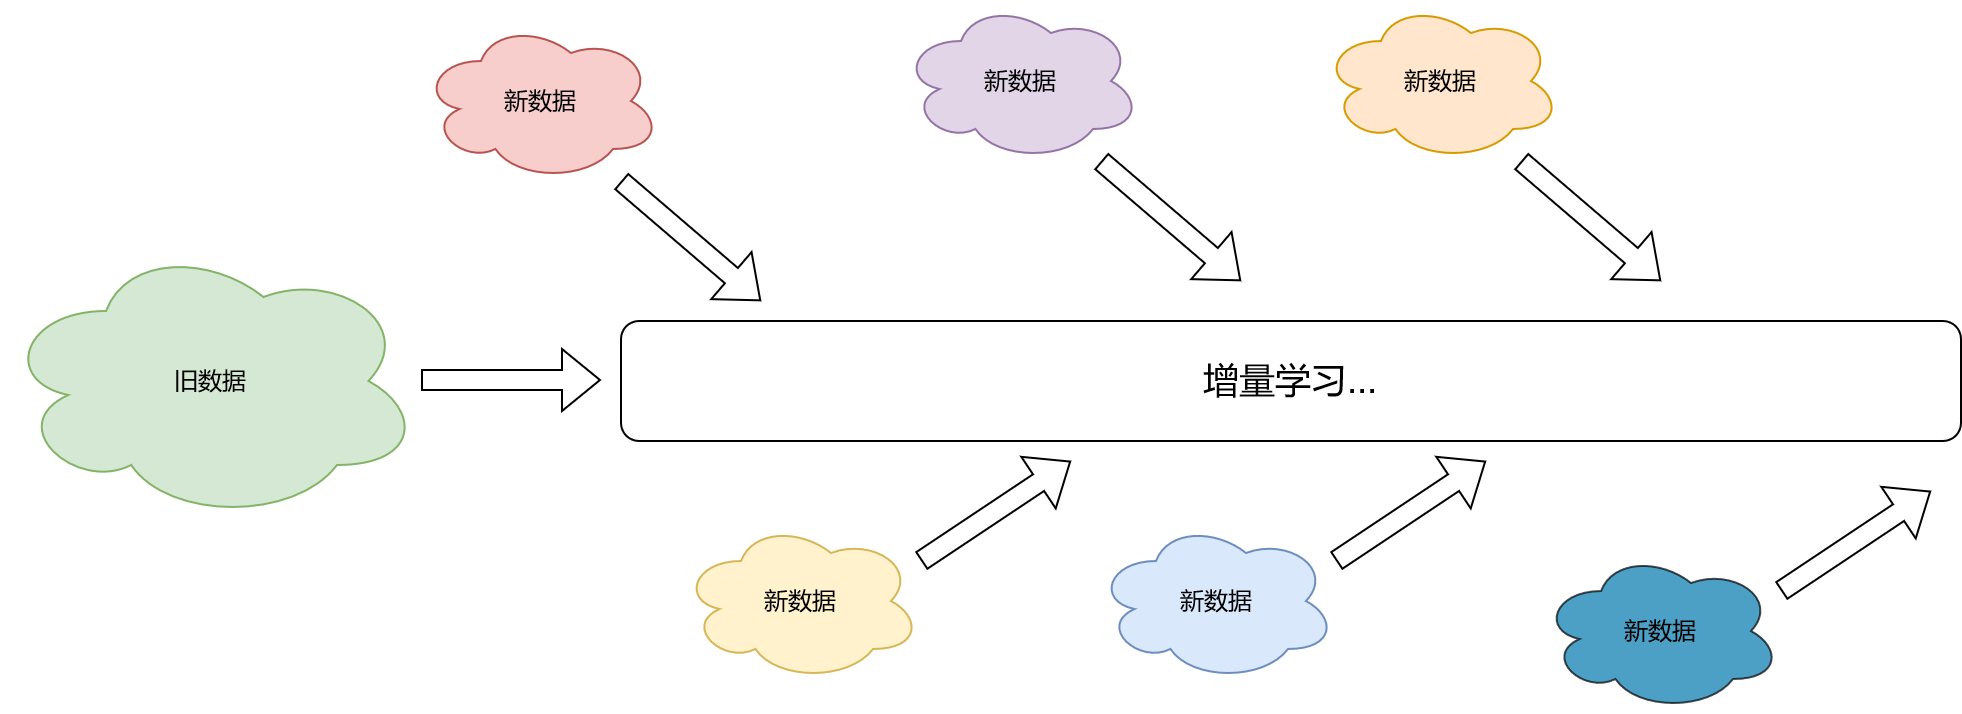
\includegraphics[width=0.9\textwidth]{increment_learning.drawio.png}
	\caption{增量学习原理图}
	\label{fig:incremental_learning}
\end{figure}
具体而言,增量学习允许模型在保留已学习知识的基础上,持续地吸收新信息并更新其知识库。

\subsection{方案具体设计}
iCaRL(Incremental Classifier and Representation Learning)\cite{rebuffi2017icarl}是一种经典的基于回放的增量学习策略。
基于回放的增量学习的基本思想就是“温故而知新”,即在接受新任务的训练过程中,同时回顾一部分精选的旧数据,以此来保持模型对先前学习任务的记忆。
因此,决定保留哪些旧任务数据以及如何有效地结合旧数据和新数据进行模型训练,是这类方法需要考虑的主要问题。\par

iCaRL的一般步骤为数据特征的学习、记忆集的管理,以及通过知识蒸馏减轻模型的遗忘。
当面对新的数据批次时,iCaRL首先结合这些新数据和从记忆集中选出的代表性样本来更新模型。
记忆集是由每个已知类别中挑选出的一小部分样本构成,旨在代表整个类别的特征分布。
通过在训练过程中包含这些样本,模型可以重新回顾已学习的类别,从而在学习新知识的同时,尽量减少对旧知识的遗忘。
接着,iCaRL通过一个更新的特征提取器来获取数据的特征表示,并利用这些特征来进行分类学习。
在学习新类别的同时,iCaRL使用知识蒸馏来保持对过去学习内容的记忆。
通过将旧模型对同一数据的输出作为额外的训练目标,新模型能够在吸收新信息的同时,减少对旧信息的遗忘。
分类决策在iCaRL中是通过计算样本与每个类别的代表性样本(即记忆集中的样本)的平均特征向量(即类中心见公式\ref{eq:class_means})之间的距离来进行的。
\begin{equation}
	\label{eq:class_means}
	\mu_c = \frac{1}{|P_c|} \sum_{p \in P_c} f(p)
\end{equation}
\begin{flushleft}
	\renewcommand\arraystretch{1.25}
	\begin{tabularx}{\textwidth}{@{}>{\normalsize\rm}l@{\quad}>{\normalsize\rm}l@{——}>{\normalsize\rm}X@{}}
		式中 & $P_c$  & 表示类别$c$的样本集; \\
		     & $f(p)$ & 样本$p$的特征表示。   \\
	\end{tabularx}\vspace{.5ex}
\end{flushleft}
分类决策的公式如式~\ref{eq:class_dist}~所示。
\begin{equation}
	\label{eq:class_dist}
	\hat{y} = \arg\min_{c \in C} \|f(x) - \mu_c\|_2
\end{equation}
\begin{flushleft}
	\renewcommand\arraystretch{1.25}
	\begin{tabularx}{\textwidth}{@{}>{\normalsize\rm}l@{\quad}>{\normalsize\rm}l@{——}>{\normalsize\rm}X@{}}
		式中 & $\hat{y}$          & 表示预测的类别;                                  \\
		     & $|f(x) - \mu_c|_2$ & 测试样本特征表示与类别$c$的类中心之间的欧氏距离。 \\
	\end{tabularx}\vspace{.5ex}
\end{flushleft}
这种基于最近中心的方法简单有效,因为它直接使用了模型学习到的特征表示来进行类别的判断。

最后,更新记忆集是iCaRL算法中一个至关重要的步骤。
随着新类别的加入,算法必须在有限的记忆容量中做出取舍,选择哪些样本继续保留在记忆集中。
这通常会涉及到对每个类别进行均衡的考虑,确保模型能够公平地回顾所有已知类别,而不是偏向于某些特定的类别。\par

基于此策略,本文接下来会将提出的RB-MF模型整合到iCaRL框架中,进而赋予其增量学习的能力。
融合RB-MF模型的iCaRL策略实现伪代码如表~\ref{tab:RB-MF-icarl}~所示。
\begin{table}[htbp]
	\caption{融合RB-MF模型的iCaRL}
	\label{tab:RB-MF-icarl}
	\centering
	\begin{tabularx}{1.0\textwidth}{cl}
		\toprule
		\multicolumn{2}{l}{\textbf{融合RB-MF模型的iCaRL策略实现}}                                                    \\
		\midrule
		\multicolumn{2}{l}{\textbf{输入}: 训练序列中的一系列数据集 $\{D_1, D_2, ..., D_n\}$,每个类别保留的样本数 $m$} \\
		\multicolumn{2}{l}{\textbf{输出}: 训练好的RB-MF特征提取器 $f_{\theta}$,更新后的记忆集 $M$}                  \\
		1  & 初始化记忆集 $M$ 为空                                                                                     \\
		2  & 初始化RB-MF特征提取器 $f_{\theta}$                                                                      \\
		3  & $for$ 每个新的数据集 $D_t$:                                                                               \\
		4  & \quad\quad $D'_t = D_t \cup M$     \Comment{合并新任务数据集和记忆集}                                     \\
		5  & \quad\quad 如果 $t > 1$,即不是处理第一个数据集:                                                          \\
		6  & \quad\quad\quad\quad 使用$f_{\theta}$的旧版本对$x$进行前向传播,得到旧类别的输出$logits_{old}$            \\
		7  & \quad\quad\quad\quad 使用知识蒸馏损失和分类损失来更新 $f_{\theta}$:                                       \\
		8  & \quad\quad\quad\quad\quad\quad $L = (1 - \alpha) L_{CE} + \alpha L_{KD}$                                  \\ %\Comment{L:整体损失,$L_{CE}$:蒸馏损失,$L_{KD}$:标准交叉熵损失} 
		9  & \quad\quad 否则,如果是处理第一个数据集:                                                                  \\
		10 & \quad\quad\quad\quad 仅使用分类损失来训练 $f_{\theta}$                                                    \\
		11 & \quad\quad $for$ 每个类别 $c=1$ 到 $n$:                                                                   \\
		12 & \quad\quad\quad\quad 从属于类别$c$的数据集$D_c$中提取所有样本$\{x_1, x_2, ..., x_k\}$                     \\
		13 & \quad\quad\quad\quad 使用当前的特征提取器网络$f_{\theta}$计算每个样本的特征表示                           \\
		14 & \quad\quad\quad\quad 计算类别$c$的特征均值向量$\mu_c$                                                     \\
		15 & \quad\quad\quad\quad 选择$m$个样本存入$M$,基于样本对特征空间的覆盖范围                                   \\
		16 & \quad\quad 对于记忆集$M$中的每个类别$c$:                                                                  \\
		17 & \quad\quad\quad\quad 计算类别$c$的特征表示的均值(类中心)$\mu_c$                                         \\
		18 & \quad\quad 当需要对新样本$x$进行分类时:                                                                   \\
		19 & \quad\quad\quad\quad 使用$f_{\theta}$计算x的特征表示$f(x)$                                                \\
		20 & \quad\quad\quad\quad 计算$f(x)$与每个类中心$\mu_c$之间的距离                                              \\
		21 & \quad\quad\quad\quad 将$x$分类到距离最近的类中心所代表的类别                                              \\
		\bottomrule
	\end{tabularx}
\end{table}

\subsection{基于遗传算法的记忆集优化抽样策略}
在进行增量学习的过程中,每当遇到新的流量类别时,模型就必须在有限的记忆空间内作出取舍。
这就需要确定每个类别的样本在记忆集中应保留的数量或比例,因此对记忆集内各类样本的有效抽样变得十分关键。
虽然传统的iCaRL策略倾向于采用均衡抽取的方法,即平等地从各个类别中抽取样本以保持类别间的平衡,但这种方法并不总能保证模型训练后的分类效果达到最佳。
这是因为不同类别的样本对于模型学习的贡献度并不相同,简单的均衡抽样可能无法充分考虑到样本对模型性能的实际影响。
针对这一问题,本小节提出了基于遗传算法的记忆集优化抽样策略。
遗传算法是一种模拟自然选择和遗传机制的搜索算法,它通过迭代进化找到问题的最优解。
在iCaRL的上下文中,遗传算法被用来优化记忆集中各个类别样本的保留比例,目标是在有限的记忆空间内最大化模型的分类性能。
对于遗传算法,本文已在第~\ref{eq:GA}~章介绍,这里不再赘述,只给出具体实施细节。\par

1)~遗传算法的选择\par
遗传算法的种类以及策略多种多样,在这里本文选择采用稳态遗传算法(Steady State Genetic Algorithm, SSGA)作为优化策略。
与传统的遗传算法相比,稳态遗传算法的特点在于每次迭代只替换种群中的一小部分个体,而不是进行全种群的更新。
这种方法的优势在于绝大多数个体在迭代过程中保持不变,从而避免了每次迭代都进行完整的种群更换。\par

考虑到本文中个体适应度评估的复杂性——每个个体的评估需要经过完整的模型训练及性能评估过程——采用标准遗传算法(即采用完全生成替换策略的遗传算法,其中每次迭代都替换整个种群)将显著增加计算负担,并可能不利于优良基因的保留。
相反,稳态遗传算法通过每次只替换部分种群的策略,不仅大幅度降低了计算量,而且有助于保持种群中的优秀个体。
这种策略的实施有助于加速算法的收敛过程,并且,通过有效地保留高质量的解,稳态遗传算法能够在全局搜索和局部搜索之间取得更好的平衡,从而提高发现全局最优解的可能性。\par

2)~特征编码\par
本文使用遗传算法搜索的目标是确定每个类别的样本在记忆集中应保留的数量或比例以便模型能够达到最佳分类效果。
为了实现这一目标,本文将会利用样本类型的抽样比重来进行特征编码。
遗传算法的每个个体(或称为“染色体”)代表一种可能的样本选择方案,其中包含了对应于数据集中每种样本类型的抽样比重。
这些比重被编码为位于$[0,1)$区间的小数,分别表示各类型样本在总体抽样策略中的比重。\par
以UNSW-NB15数据集为例,一个可能的染色体编码可以是{0.2, 0.3, 0.1, 0.5, 0.3,0.1,0.2,0.1,0.4,0.1},这分别对应于十种样本类型的采样比重。
需要注意的是,这些比重在实际应用中将会具体调整为抽样百分比。
在进行实际训练时,通过计算记忆集样本数量与各类样本抽样百分比的乘积,便可得到每类样本具体的抽样数量。
例如,对于样本数量为1,000的记忆集,该染色体对应的每类样本采样百分比、采样数量如表~\ref{tab:Ga_code}~所示。\par
\begin{table}[h]
	\caption{遗传算法编码方案}
	\label{tab:Ga_code}
	\centering
	\begin{tabular}{cccc}
		\toprule
		\textbf{编码值(基因)} & \textbf{样本类型} & \textbf{采样百分比} & \textbf{抽样数量} \\
		\midrule
		0.2                   & normal            & 8.695652\%          & 87                \\
		0.3                   & Fuzzers           & 13.043478\%         & 130               \\
		0.1                   & Recon             & 4.347826\%          & 44                \\
		0.5                   & Shellcode         & 21.73913\%          & 217               \\
		0.3                   & Analysis          & 13.043478\%         & 130               \\
		0.1                   & Backdoors         & 4.347826\%          & 44                \\
		0.2                   & DoS               & 8.695652\%          & 87                \\
		0.1                   & Exploits          & 4.347826\%          & 44                \\
		0.4                   & Generic           & 17.391304\%         & 174               \\
		0.1                   & Worms             & 4.347826\%          & 43                \\
		\bottomrule
	\end{tabular}
\end{table}

3)~适应度评估\par
在本文中将会利用基因对应的抽样比率对训练集进行分层抽样,并利用RB-MF模型在增强后的记忆集上进行训练。
最后再在验证集上使用accuracy\_score(公式~\ref{eq:val_score1}~)作为评价标准进行评估,评估值便作为该染色体对应的适应度。\par

4)~初始群体生成及迭代次数\par
为了确保算法能够充分探索解空间并增加解的多样性,本文特别注重初代种群基因的广泛性和迭代过程的深入性。
基于此目的,初始种群规模被设定为1,000个个体,从而覆盖更广泛的解空间、提高找到全局最优解的概率。
同时,为了充分优化解并观察算法的收敛行为,设置了10,000次的迭代次数,以便于算法有足够的时间逐步改进解,并最终接近最优解。\par

5)~选择、交叉和变异\par
对于选择策略,本文采用轮盘赌选择法,该方法根据个体适应度相对于总体适应度的比例来分配选择概率。
这种方法的优势在于能够有效保证高适应度个体被优先选择,从而引导种群朝着更优解空间方向进化。
在交叉操作方面,为了降低计算的复杂度,本文选择了单点交叉方法。
对于变异策略,本研究设置了0.1的固定概率对新生成的个体中的所有基因进行变异。
在确定变异位置后,以相等的概率选择将该基因值进行1.2倍的放大或0.8倍的缩小。
这样做的目的是保证个体的基因以较小的变化幅度进行细微调整,增强种群的探索能力,同时避免过大的变异导致优秀基因的丢失。
表~\ref{tab:genetic_algorithm}~是本文遗传算法实现的伪代码。
\begin{table}[h]
	\caption{遗传算法实现}
	\label{tab:genetic_algorithm}
	\centering
	\begin{tabularx}{1.0\textwidth}{cl}
		\toprule
		\multicolumn{2}{l}{\textbf{遗传算法}}                                               \\
		\midrule
		\multicolumn{2}{l}{\textbf{输入}: 种群大小 $P$,基因数量 $G$,代数 $N$,变异率 $M$} \\
		\multicolumn{2}{l}{\textbf{输出}: 最优染色体}                                       \\
		1  & 初始化种群(population)                                                         \\
		2  & \textbf{for} generation \textbf{in} $N$:                                       \\
		3  & \quad \textbf{for} individual \textbf{in} population:                          \\
		4  & \quad\quad \#依据个体基因对应的抽样比率进行抽样                                \\
		5  & \quad\quad train\_set = sampling(train\_set,gene)                              \\
		6  & \quad\quad train(model, train\_set)                                            \\
		7  & \quad\quad fitness = evaluate(model, test\_set)                                \\
		8  & \quad \#根据个体适应度利用轮盘赌选择法进行选择                                 \\
		9  & \quad $p1, p2$ = select\_parents(population, fitness)                          \\
		10 & \quad $c1, c2$ = crossover($p1, p2$)                                           \\
		11 & \quad mutate($c1$), mutate($c2$) with rate $M$                                 \\
		12 & \quad add $c1, c2$ to population                                               \\
		13 & \quad update\_fitness(population)                                              \\
		14 & \quad \#根据个体适应度对应的淘汰概率利用轮盘赌选择法进行淘汰                   \\
		15 & \quad eliminate\_individuals(population,fitness)                               \\
		16 & \textbf{return} highest\_fitness\_chromosome(population)                       \\
		\bottomrule
	\end{tabularx}
\end{table}


\subsection{实验评估}
\textbf{1.数据集介绍}\par
KDD Cup 99数据集\cite{tavallaee2009detailed}曾长期被视为网络入侵检测研究的标准化数据集。
然而,该数据集存在一些明显的局限性,例如庞大的数据量和大量的冗余记录,这些因素共同导致了模型训练和测试的效率低下。
为了解决这些问题并提高研究效率,NSL-KDD数据集\cite{revathi2013detailed}应运而生,它在网络安全领域得到了广泛的应用和认可。
NSL-KDD数据集的设计旨在消除冗余性、改善平衡性、增加多样性和扩展适用性。
通过剔除KDD Cup 99数据集中的冗余记录,NSL-KDD数据集显著缩减了数据规模,不仅大幅提升了模型和算法的训练效率,使其能在更短的时间内完成训练过程,还有效降低了因数据冗余可能导致的偏差风险,进一步增强了模型的稳定性和准确性。
尽管NSL-KDD并未完全解决数据类别不平衡的问题,但相较于其前身,它在一定程度上减轻了这一问题,为研究人员提供了一个更加平衡的数据环境。\par

NSL-KDD数据集由41个特征组成,整体包括八个文件,分成四组数据,每组提供了两种格式:文本文件格式(.txt)和属性关系文件格式(.arff)。
这些文件的详细描述如表~\ref{tab:NSLKDDFile}~所示。
\begin{table}[htbp]
	\caption{NSL-KDD数据集各文件介绍}
	\label{tab:NSLKDDFile}
	\begin{tabularx}{\textwidth}{cXc}
		\toprule
		\textbf{文件名}         & \textbf{描述}                                                  & \textbf{记录总数} \\
		\midrule
		KDDTrain+.ARFF          & 完整的NSL-KDD训练集以二进制标签的ARFF格式提供                  & 125973            \\
		KDDTrain+.TXT           & 完整的NSL-KDD训练集,包括攻击类型标签和难度级别,以CSV格式提供 & 125973            \\
		KDDTrain+20Percent.ARFF & KDDTrain+.arff文件的20\%子集                                   & 25192             \\
		KDDTrain+20Percent.TXT  & KDDTrain+.txt文件的20\%子集                                    & 25192             \\
		KDDTest+.ARFF           & 完整的NSL-KDD测试集以二进制标签的ARFF格式提供                  & 22544             \\
		KDDTest+.TXT            & 完整的NSL-KDD测试集,包括攻击类型标签和难度级别,以CSV格式提供 & 22544             \\
		KDDTest-21.ARFF         & 不包含难度级别为21的记录的KDDTest+.arff文件的子集              & 11850             \\
		KDDTest-21.TXT          & 不包含难度级别为21的记录的KDDTest+.txt文件的子集               & 11850             \\
		\bottomrule
	\end{tabularx}
\end{table}
NSL-KDD数据集中包含的攻击流量可分为拒绝服务攻击(DoS)、远程到本地攻击(R2L)、用户到根攻击(U2R)以及探测攻击(Probe)共四种类别。
如表~\ref{tab:attack_class}~所示,这四种类别又可细分为39种子类型。
\begin{table}[h]
	\caption{NSL-KDD数据集中每种攻击的不同子类的细分}
	\label{tab:attack_class}
	\begin{tabularx}{\textwidth}{@{}ccX@{}}
		\toprule
		\multicolumn{1}{c}{\textbf{种类}} & \multicolumn{1}{c}{\textbf{数量}} & \multicolumn{1}{c}{\textbf{子类}}                                                                                                                \\
		\midrule
		DoS                               & 11                                & apache2, back, land, neptune, mailbomb, pod, processtable, smurf, teardrop, dupstorm, worm                                                       \\
		Probe                             & 6                                 & ipsweep, mscan, nmap, portsweep, saint, satan                                                                                                    \\
		U2R                               & 7                                 & buffer\_overflow, loadmodule, perl, ps, rootkit, sqlattack, xterm                                                                                \\
		R2L                               & 15                                & ftp\_write, guess\_passwd, httptunnel, imap, multihop, named, phf, sendmail, snmpattack, spy, snmpguess, warezclient, warezmaster, xlock, xsnoop \\
		\bottomrule
	\end{tabularx}
\end{table}
表~\ref{tab:kdd_distribution}~则展示四种类别的攻击流量与正常流量在数据集中的分布占比。
\begin{table}[h]
	\caption{每种攻击类型的数据分布}
	\label{tab:kdd_distribution}
	\centering
	\begin{tabular}{ccccccc}
		\toprule
		\textbf{数据集}                & \textbf{总数}           & \textbf{Normal} & \textbf{DoS} & \textbf{Probe} & \textbf{R2L} & \textbf{U2R} \\
		\midrule
		\multirow{2}{*}{KDDTrain+}     & \multirow{2}{*}{125973} & 67343           & 45927        & 11656          & 995          & 52           \\
		                               &                         & 53.46\%         & 36.46\%      & 9.25\%         & 0.79\%       & 0.04\%       \\
		\multirow{2}{*}{KDDTest+}      & \multirow{2}{*}{22544}  & 9711            & 7636         & 2423           & 2574         & 200          \\
		                               &                         & 43.08\%         & 33.87\%      & 10.74\%        & 11.42\%      & 0.89\%       \\
		\multirow{2}{*}{KDDTrain+20\%} & \multirow{2}{*}{25192}  & 13449           & 9234         & 2289           & 209          & 11           \\
		                               &                         & 53.39\%         & 36.65\%      & 9.09\%         & 0.83\%       & 0.04\%       \\
		\bottomrule
	\end{tabular}
\end{table}
图~\ref{fig:kddtraindistribution}~、~\ref{fig:kddtestdistribution}~分别是完整训练集与测试集中各种流量分布占比饼状图。
\begin{figure}[htbp]
	\centering
	\subcaptionbox{训练集\label{fig:kddtraindistribution}}[0.4\textwidth]{
		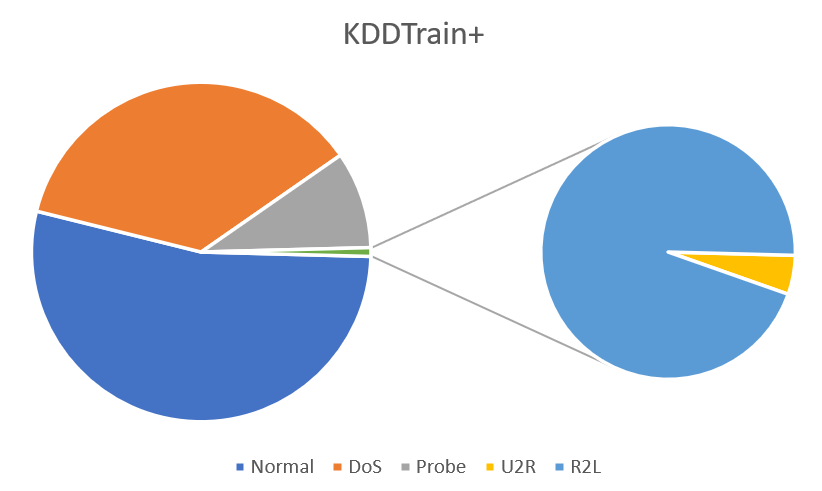
\includegraphics[width=0.4\textwidth]{kddtraindistribution.png}
	}
	\hspace{36pt}
	\subcaptionbox{测试集\label{fig:kddtestdistribution}}[0.4\textwidth]{
		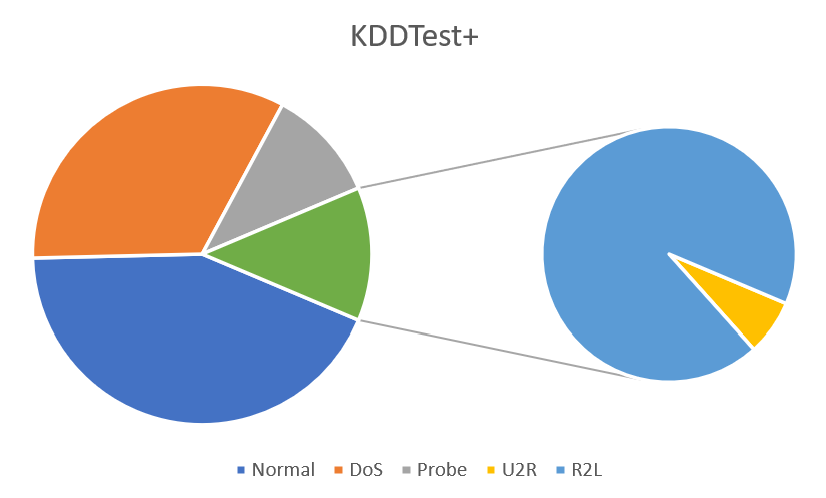
\includegraphics[width=0.4\textwidth]{kddtestdistribution.png}
	}
	\caption{NSL-KDD完整数据集分类占比饼状图}
\end{figure}

通过以上图表可知数据集中不同攻击类型的数据分布不均衡,特别是U2R和R2L攻击类型的样本数量远少于其他类型。
这种不平衡分布对于训练入侵检测系统模型来说是一个挑战,因为模型可能会在较多样本的攻击类型上表现更好,而在样本较少的攻击类型上表现不佳。
此外,从KDDTrain+到KDDTest+,攻击类型的分布变化表明,测试集可能代表了与训练集不同的攻击环境,这要求模型具备良好的泛化能力,以适应不同的攻击行为和模式。\par

\textbf{2.实验设计}\par
本文首先使用UNSW-NB15作为旧任务数据集,并将其划分为训练集和测试集。
具体而言,本文选取数据集中的80\%作为训练集,用于训练模型以获取基本的网络攻击检测能力;剩余的20\%则作为测试集,用于初步评估模型的性能。
随后,本文直接利用NSL-KDD提供的训练集文件中的数据作为新任务数据集,同时采用NSL-KDD提供的测试集文件中的数据作为测试集。
为了进行增量学习,本文采用批量读取的方式处理新任务数据集。
每个增量学习阶段设定读取1,000个样本,同时设定记忆集的大小与每阶段训练集的大小保持一致,均为1,000。
在增量学习的每个批次中,本文都进行100轮的训练,以确保模型能够充分学习当前批次的数据。\par

\textbf{3.实验结果与分析}\par
为验证本文方案进行增量学习后的效果,本文选取了一系列模型,包括DT(决策树)、LR(逻辑回归)、KNN(K近邻)、NB(朴素贝叶斯)、Ada(AdaBoost增强)、ResN(残差神经网络)、BiG(双向门控循环单元)、RB-NMF(未经多模态特征融合的残差神经网络与双向门控循环单元)、RB-MF(经过多模态特征融合的残差神经网络与双向门控循环单元)、RB-MF with iCaRL(基于iCaRL的RB-MF模型),以及RB-MF with iCaRL and GA(结合了遗传算法记忆集抽样优化的RB-MF with iCaRL模型),并对这些模型进行了增量学习实验。
当所有新任务训练集的内容学习完成后,本文将新任务测试集与旧任务测试集进行合并形成混合测试集,用以评估各模型在混合数据集上的性能。\par

图~\ref{fig:acc_icarl}展示了各个模型在混合测试集上的准确率表现。
\begin{figure}[h]
	\centering
	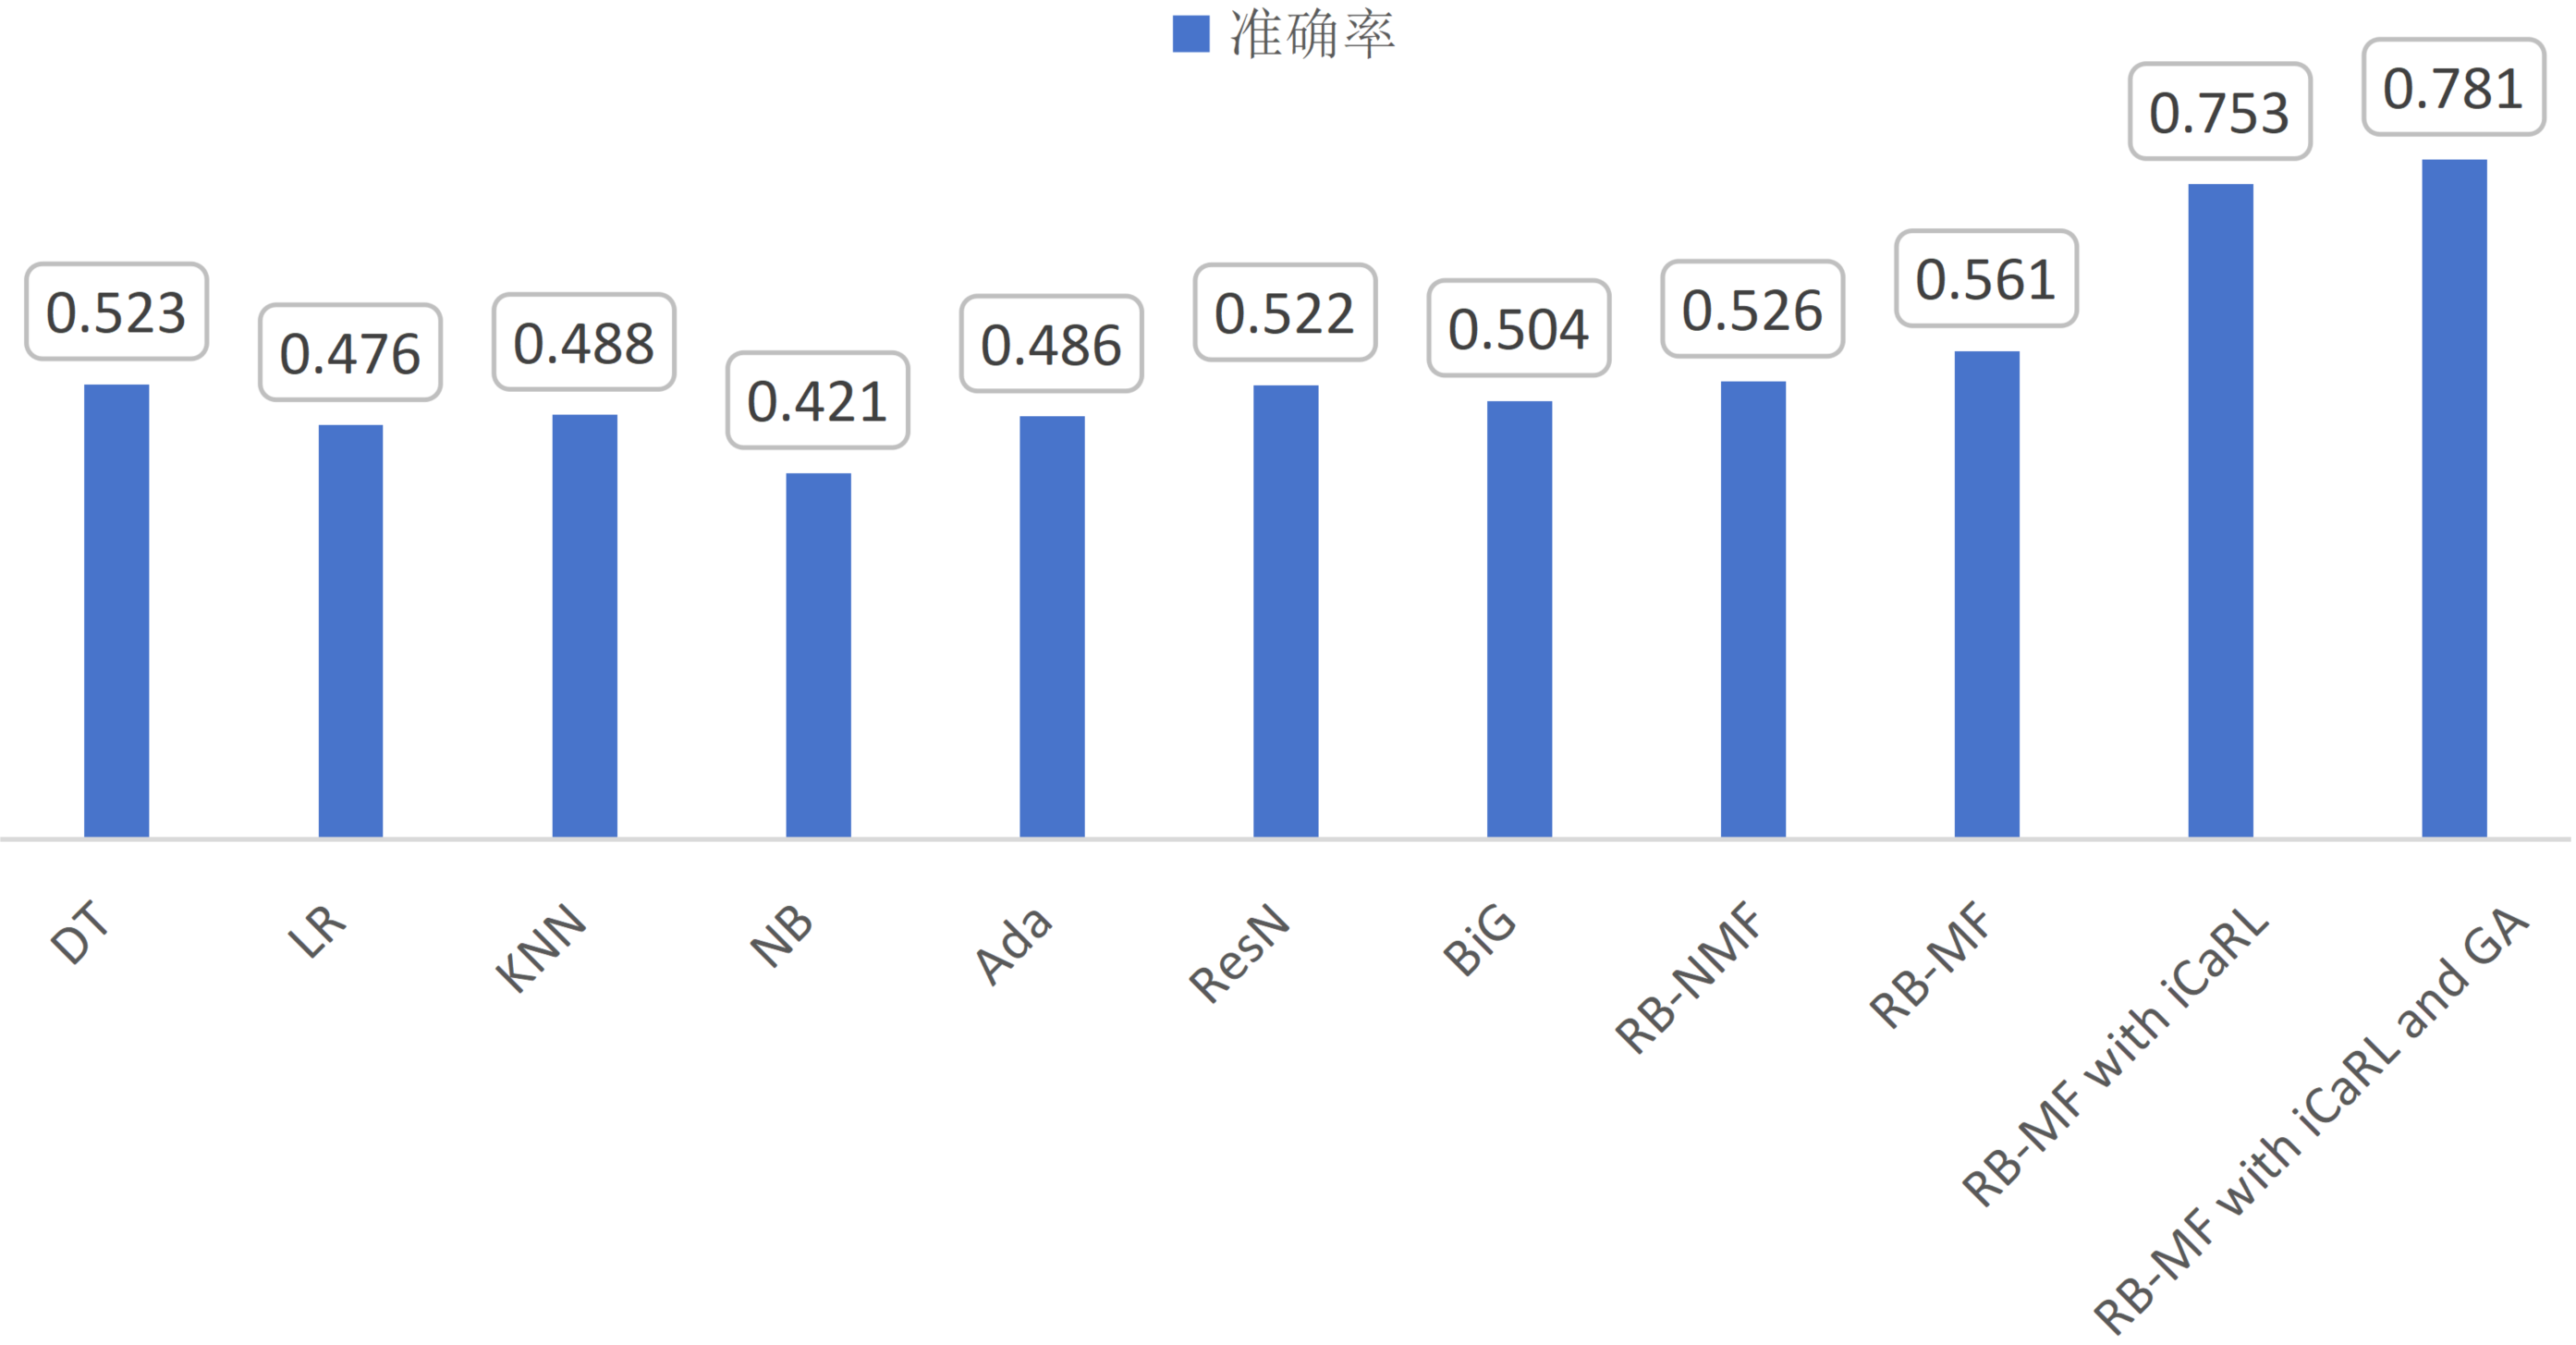
\includegraphics[width=0.8\textwidth]{icarl_accuracy.png}
	\caption{增量学习后各模型在混合测试集上准确率对比柱状图}
	\label{fig:acc_icarl}
\end{figure}
从图中可以明显看出,引入iCaRL策略后,模型的检测准确率得到了显著提升。
这一结果充分证明了iCaRL策略在保持模型对旧知识记忆的同时学习新知识的有效性。
特别值得注意的是,本文提出的基于遗传算法的记忆集抽样优化方法在iCaRL的基础上进一步提高了RB-MF模型的准确率。
这表明该方法能够有效保留模型的记忆能力,提升其在增量学习过程中的性能。
然而,对于未引入iCaRL策略的其他模型,例如机器学习模型以及深度学习模型如ResNet(ResN)和BiG等,在进行增量学习后的表现并不尽如人意。
这可能是因为这些模型在学习新知识的过程中,容易遗忘旧知识,导致在混合测试集上的性能下降。
下面的实验是对这一问题的具体验证。

图~\ref{fig:acc_forget}是每十个增量学习阶段后模型在旧任务数据集上的准确率变化。
\begin{figure}[h]
	\centering
	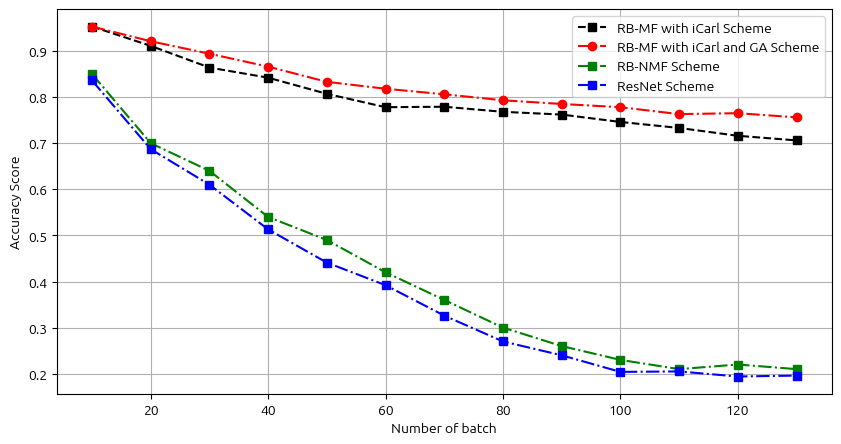
\includegraphics[width=0.8\textwidth]{forget.png}
	\caption{增量学习后模型在旧任务数据集上的准确率下降对比柱状图}
	\label{fig:acc_forget}
\end{figure}
\par
从图中可以看出,没有结合iCaRL策略的模型在经过增量学习后,其准确率迅速下降,
而结合了iCaRL策略的RB-MF模型则能够较好地保持准确率,最终模型的准确率保持在70\%以上。
这表明模型在没有采取额外策略的情况下学习新知识会导致对旧知识的遗忘。
特别值得一提的是,当使用本文所提出的基于遗传算法的记忆集抽样优化策略后,模型的准确率仍能得到进一步的提升。
这表明了本文提出的记忆集抽样优化策略能有效增强模型的增量学习效果。

\section{本章小结}
在本章中,本文提出了一种多模态特征融合模型,该模型基于残差网络与双向门控循环单元,旨在提升传统网络攻击检测技术的准确性。
通过在实验数据集上与多种经典机器学习和深度学习模型进行详尽的对比分析,本文的模型展现出了显著的性能优势。
为了进一步应对不断变化的网络攻击环境带来的挑战,本文引入了iCaRL技术,设计了一种基于多模态特征融合的增量学习方案。
这一方案旨在确保模型在维持对原有网络攻击的高效识别能力的同时,不断适应并学习新型的网络攻击模式。
通过持续的学习,本文的模型能够更好地应对不断变化的网络环境,提升整体的安全防护能力。
此外,本文针对增量学习过程中使用的记忆集,提出了一种基于遗传算法的抽样优化方法。
这一方法能够更加高效地利用有限的资源,提升增量学习的效率和准确性。
在实验中,本文以UNSW-NB15与NSL-KDD分别作为新旧数据集,与多种经典机器学习和深度学习模型进行了对比分析。
实验结果表明,本文的增量学习方案能够显著增强模型的学习能力,实现了对旧知识的有效保留和新知识的快速学习。